% Template for Part III essays 2024/25 (12.02.2025)
% Authors: Mycroft Rosca-Mead, Matt Colbrook, Jonathan Evans.

%%%%%%%%%%%%%%%%%%%%%%%%%%%%%%%%%%%%%%%%%%%%%%%%%%%%%%%%%%%%%%%%%%%%%%

% The following few lines are preliminaries and MUST NOT BE EDITED
\documentclass[11pt, titlepage]{article} % DO NOT CHANGE THE FONT SIZE
\usepackage[left=2.2cm,right=2.2cm,top=2.5cm,bottom=2.5cm]{geometry} % DO NOT CHANGE THE MARGINS
\usepackage{amsfonts,amssymb,amsthm,amsmath,amscd,bbm}
\usepackage{enumerate}
\usepackage{tikz}
\usetikzlibrary{trees,positioning,calc}

%%%%%%%%%%%%%%%%%%%%%%%%%%%%%%%%%%%%%%%%%%%%%%%%%%%%%%%%%%%%%%%%%%%%%%

% ESSAY TITLE
% Your essay title should match the title given in the essay booklet.
% If you wish to give the essay your own subtitle, you can do this after the title page (e.g. using \section*{Subtitle Name}).
% You do not need to use \Author and YOU SHOULD NOT INCLUDE YOUR NAME OR COLLEGE ANYWHERE IN THIS ESSAY.
% The title page does not count towards the total page number.
\title{Points of Infinite Multiplicity of Planar Brownian Motion}

% DATE
%To remove the date from the front page of the final version, UNCOMMENT the line below.
\date{}

% FONTS
%\renewcommand{\familydefault}{\sfdefault}
% YOU MUST USE EITHER THE SANS-SERIF FONT DEFINED BY THE COMMAND ABOVE OR THE STANDARD LaTeX (computer modern) FONT THAT CAN BE OBTAINED BY COMMENTING OUT THE LINE ABOVE. YOU MUST NOT USE ANY OTHER FONT.

%%%%%%%%%%%%%%%%%%%%%%%%%%%%%%%%%%%%%%%%%%%%%%%%%%%%%%%%%%%%%%%%%%%%%%
% A guide to using LaTeX can be found online at https://www.overleaf.com/learn/latex/Learn_LaTeX_in_30_minutes.
% A shorter LaTeX cheat sheet can be found at https://wch.github.io/latexsheet/.

%%%%%%%%%%%%%%%%%%%%%%%%%%%%%%%%%%%%%%%%%%%%%%%%%%%%%%%%%%%%%%%%%%%%%%
% Some latex tips:

% Use this space for any special macros or packages you need.
\usepackage{graphicx}

% use this package for easy referencing:
\usepackage{overpic} % use this package for easy labelling of figures
\usepackage{url} % use this package to reference urls, e.g., \url{https://www.maths.cam.ac.uk/postgrad/part-iii/prospective.html}
\usepackage{comment} % use this package to comment things out \begin{comment} blah \end{comment}
\usepackage[colorlinks=true, linkcolor=blue, citecolor=blue, urlcolor=blue]{hyperref}
\usepackage[capitalise,noabbrev]{cleveref} % e.g., \cref{amazing_theorem} will reference "`Theorem"' X without having to keep track of theorems, equations etc and typing "`Theorem"'

% FIGURES
% Here is an example of how to do figures:

%\begin{figure}
%\centering
%\includegraphics[width=\linewidth]{CMS at night_0.jpg}
%\caption{The CMS at night.}\label{fig:cms}
%\end{figure}

% General tip: Many tex problems can be easily solved by a quick and specific google search.


%%%%%%%%%%%%%%%%%%%%%%%%%%%%%%%%%%%%%%%%%%%%%%%%%%%%%%%%%%%%%%%%%%%%%%
%FOOTNOTES
\newcommand\blfootnote[1]{% avoids footnotes spilling over
  \begingroup
  \renewcommand\thefootnote{}\footnote{#1}%
  \addtocounter{footnote}{-1}%
  \endgroup
}

%%%%%%%%%%%%%%%%%%%%%%%%%%%%%%%%%%%%%%%%%%%%%%%%%%%%%%%%%%%%%%%%%%%%%%
% The following relate to equations, theorems, etc, as illustarted in the document. 

\numberwithin{equation}{section}
% EQUATION NUMBERING: The command above can be changed to number equations within subsections, rather than sections, or it can be commented out to number equations through the document, irrespective of (sub)sections.

\newtheorem{theorem}{Theorem}
\newtheorem{lemma}{Lemma}
\newtheorem{corollary}{Corollary}
\newtheorem{proposition}{Proposition}
\newtheorem{definition}{Definition}
\theoremstyle{definition}
\newtheorem{remark}{Remark}
\newtheorem{example}{Example}

\numberwithin{theorem}{section}
\numberwithin{lemma}{section}
\numberwithin{corollary}{section}
\numberwithin{proposition}{section}
\numberwithin{definition}{section}
\numberwithin{remark}{section}
% NUMBERING OF THEOREMS ETC: The commands above can be changed to number within subsections, rather than sections, or commented out to number them through the document, irrespective of (sub)sections.

%%%%%%%%%%%%%%%%%%%%%%%%%%%%%%%%%%%%%%%%%%%%%%%%%%%%%%%%%%%%%%%%%%%%%%
% Shortcuts for commonly used symbols
\newcommand{\R}{\mathbb{R}}
\newcommand{\N}{\mathbb{N}}
\newcommand{\Z}{\mathbb{Z}}
\newcommand{\Q}{\mathbb{Q}}
\newcommand{\C}{\mathbb{C}}
\newcommand{\ind}{\mathbbm{1}}
\newcommand{\expect}{\mathbb{E}}
\newcommand{\prob}{\mathbb{P}}
\newcommand{\Cantor}{\mathfrak{C}}
\renewcommand{\L}{\mathcal{L}}
\newcommand{\deq}{{\buildrel d \over =}}
\newcommand{\defeq}{\mathrel{\mathop:}=}

%%%%%%%%%%%%%%%%%%%%%%%%%%%%%%%%%%%%%%%%%%%%%%%%%%%%%%%%%%%%%%%%%%%%%%
\begin{document}
\maketitle
%%%%%%%%%%%%%%%%%%%%%%%%%%%%%%%%%%%%%%%%%%%%%%%%%%%%%%%%%%%%%%%%%%%%%%

% START OF ESSAY
\tableofcontents

\section*{Notation conventions}
With the intention of making the consumption of this text as convenient as possible for the reader, let us introduce some common notation that will be used throughout this document.

We will denote with $\mathcal{B}(X)$ the Borel sets of a topological space X. We will also write $\R_\geq=\{t\in\R:t\geq0\}$, and equivalently for $\R_>, \R_\leq,\text{ and } \R_<$. For a subset $A\subseteq\R^n$, we similarly write $A_\leq=\{(t_1,\dots,t_n)\in A: t_1\leq t_2\leq\dots\leq t_n\}$, and the corresponding sets for $A_<$, $A_\geq$ and $A_>$. We will write $\mathcal{C}(A\to B)$ the set of continuous functions $f:A\to B$ for two spaces $A$ and $B$. We will work under a probability space $(\Omega, \mathcal{F}, \prob)$, and we will refer to the space of $p$-integrable measurable functions as $\mathcal{L}^p=\mathcal{L}^p(\Omega, \mathcal{F}, \prob)$, where $X$ is $p$-integrable if $\|X\|_p=(\expect[|X|^p])^{1/p}<\infty$.

We will refer to planar Brownian motion at time $t$ with $B(t)$. For $x\in\R^n$ and $r>0$ we write the open ball of radius $r$ and centre $x$ as $D_r(x)=\{y\in\R^n:\|x-y\|_n<r\}$ and the closed ball as $\bar{D}_r(x)$. We define the indicator function as 
\[
\ind_A(x)=\begin{cases}
    1 \hspace{1em}\text{if} \hspace{0.4em}x\in A \\
    0 \hspace{1em}\text{otherwise}
\end{cases}
\]
for a point $x$ in the same space as the subset $A$.

Furthermore, we will use the abbreviations RHS and LHS for `right-hand side' and `left-hand side', respectively. We will write a.s. for `almost surely', and w.p for `with probability'. Lastly, for equality in distribution we will write $\deq$.

\newpage
\section{Introduction}
Despite its simple definition, Brownian motion exhibits a very rich structure, often hiding remarkable and unintuitive properties. Its first mathematical construction is due to Norbert Wiener in 1923, but it owes its name to Robert Brown, who observed the erratic motion of pollen particles in water in 1827. Other early works in Brownian motion include the physical model developed by Einstein, and Bachelier's thesis on pricing stock options, both in the early 1900s. Paul Lévy also contributed greatly to the theory of Brownian motion with his monograph in 1958 (\cite{AdvProb},\cite{LeGallSomeProperties}).

The main objective of this essay is not to present original results, but to explore a mathematically rich and subtle topic within probability and convey it in an accessible way. The intended audience consists of students in Mathematics who are comfortable with probability and measure theory at the level of the Part III course in Advanced Probability \cite{AdvProb}. In particular, familiarity with the basic theory of Brownian motion is assumed.

Brownian motion exhibits different behaviour depending on the ambient dimension. Some of its better known properties are recurrence and transience. Linear Brownian motion is point recurrent, meaning that the set of hitting times for any point is unbounded almost surely. Planar Brownian motion, on the other hand, is point transient, i.e. it does not hit points. However, it is neighbourhood recurrent, meaning that, with probability one, it returns to a ball around any given point infinitely often (\cite{AdvProb}). This and the title of the essay raise an intriguing question: if planar Brownian motion does not hit points, in what sense can it have multiple points? We address this question by showing that, despite not hitting any individual point, it nonetheless intersects itself in such a way that certain locations are visited infinitely many times (\cite{LeGallSomeProperties}).

This essay aims to explore some machinery that makes this result precise and provable. The fundamental tools are the intersection local times,  presented in \cref{sect:local-times}. These are measures that offer a rigorous way to quantify the time Brownian paths spend intersecting each other. Their construction is technically involved and may seem opaque at first, but we will see how these objects offer deep insight into the structure of Brownian motion. Most results and ideas in this section are from \cite{LeGallSomeProperties} and \cite{RandomWalkIntersections:}. Before continuing, we end this part with a mention of local times for one dimensional Brownian motion, which are the original object that motivates their name, and was first studied by Lévy.

In the second half of the essay, in \cref{sect:multiple_points}, we study the occurrence and nature of points that are revisited by the Brownian path. This includes points of infinite multiplicity that give name to this essay, but also finite multiple points. To build intuition, we examine, in particular, double points. In this brief overview, we introduce the concept of renormalisation, which is much richer and hard to approach in general, but it is insightful in the case of double points. At this stage, our focus is to introduce the final tools necessary, and culminate all our previous efforts with a proof of almost sure existence of multiple points. This not only establishes the presence of such points, but also provides a characterisation of the structure of the set of times at which the Brownian path visits such points, which is in itself a testament to the richness and complexity of Brownian motion. The primary ideas here come from \cite{LeGallSomeProperties} and \cite{LeGallFrench}.

As a historical note, the study of intersection local times and multiple points in Brownian motion has deep roots in both probability theory and mathematical physics. The concept of intersection local time was initially motivated by physical models, with foundational contributions by Edwards, Symanzik, Varadhan, and Wolpert. Geman, Horowitz, and Rosen exploited the Gaussian nature of Brownian motion to obtain precise results. In parallel, the question of points of finite or infinite multiplicity in Brownian paths was settled through the work of Dvoretzky, Erdős, Kakutani, and Taylor. Although their proof of points of infinite multiplicity for planar Brownian motion was not complete. Le Gall introduced a new proof, which is presented here. These two topics — intersection local times and multiple points — form the core of this essay. (Bibliographical notes of chapters VIII and IX in \cite{LeGallSomeProperties})


\section{Local times}\label{sect:local-times}

\subsection{Intersection local times}
We will introduce two random measures that are central to our goal of showing that planar Brownian motion has points of arbitrary multiplicity. We will first give formal definitions of such measures, then we will construct them rigorously and provide some of their properties. Both of these measures are random Radon measures, concepts which we recall below (See \cite{RandomMeasures} Chapters 1,2, \cite{NorrisProbMeasure}).

\begin{definition}[Radon measure]
    Let $E$ be a Hausdorff topological space. A measure $\mu$ on $(E,\mathcal{B}(E))$ satisfying that $\mu(K)<\infty$ for any compact $K\in\mathcal{B}(E)$ is called a \textnormal{Radon measure} on $E$.
\end{definition}

\begin{definition}[Random measure]
    Given a probability space $(\Omega,\mathcal{F},\mathbb{P})$ and a $\sigma$-finite measurable space $(E,\mathcal{E})$, a \textnormal{random measure} X is a map $X:\Omega\times\mathcal{E}\to\bar\R$ such that $X(\omega,\cdot)$ is a measure on $E$ for any fixed $\omega\in\Omega$, and $X(\cdot,B)$ is $\mathcal{F}$-measurable for any fixed $B\in\mathcal{E}$. In particular, $X$ is called a \textnormal{kernel} from $\Omega$ to $E$.
\end{definition}

\begin{remark}
    In the measures that we will define in the following sections, the randomness comes from the sample paths of Brownian motion since their values depend on the points that the Brownian motion visits.
\end{remark}

\subsubsection{Intersection local time of independent Brownian motions}\label{sect:alpha_local_time}
For $p\geq2$, let $B_1,\dots, B_p$ be $p$ independent planar Brownian motions with arbitrary starting points $x_1,\dots,x_p$. Intuitively, our goal is to introduce a quantity that measures how much $B_1,\dots, B_p$ intersect.

\begin{definition}[Intersection local time]
The \textnormal{intersection local time} of $B_1,\dots,B_p$ is a random Radon measure $\alpha$ on $\R_\geq^p$ formally defined by:
\[
\alpha(dt_1\dots dt_p)=\left[\int_{\R^2}\prod_{j=1}^p\delta_y(B_j(t_j))dy\right]dt_1\dots dt_p,
\]
where $\delta_y$ is the Dirac delta function at y. For convenience, we write $\varphi(z_1,\dots,z_p)=\int_{\R^2}\prod_{j=1}^p\delta_y(z_j)dy$. Equivalently,
\begin{equation}\label{eq:alpha_local_time_difference_of_bs}
    \alpha(dt_1\dots dt_p)=\delta_0\left(B_1(t_1)-B_2(t_2)\right)\dots\delta_0\left(B_{{p-1}}(t_{p-1})-B_{{p}}(t_{p})\right)dt_1\dots dt_p.
\end{equation}
\end{definition}

In order to construct this measure rigorously, we start with an approximation of $\delta_y$:
\[
    \delta^\epsilon_y(z)=\frac{1}{\pi\epsilon^2}\ind_{D_\epsilon(y)}(z).
\]
Notice that for every bounded and continuous function $f$ on $\R^2$, we have
\[
\lim_{\epsilon\downarrow0}\int_{\R^2}f(x)\delta_y^\epsilon(x)dx=f(y),
\]
so the probability density function $\delta_y^\epsilon$ (weakly) converges to the Dirac delta function $\delta_y$.

For $\epsilon>0$, consider the following random measure:
\[
\alpha_\epsilon(dt_1\dots dt_p)=\varphi_\epsilon(B_1(t_1),\dots,B_p(t_p))dt_1\dots dt_p,
\]
where, 
\[\varphi_\epsilon(z_1,\dots,z_p)=\int_{\R^2}\prod_{j=1}^p\delta^\epsilon_y(z_j)dy,\] for $z_j\in\R^2$, and $j=1,\dots,p,$.


Note that for $A_1,\dots, A_p\in\mathcal{B}(\R)$ bounded we have 
\begin{equation}\label{eq:alpha_ep_local_time_formula_for_sets}
    \alpha_\epsilon(A_1\times\dots A_p)=\int_{A_1,\dots, A_p}\varphi_\epsilon(B_1(t_1),\dots,B_p(t_p))ds_1\dots ds_p=\int_{\R^2}dy\prod_{j=1}^p\int_{A_j}\delta^\epsilon_y(B_j(t_j))dt_j
\end{equation}

In the following theorem we construct the measure $\alpha$ by showing that as $\epsilon\downarrow0$, $\alpha_\epsilon$ converges on all Cartesian products of bounded Borel subsets of $\R_\geq$. Then, we will show that the limiting family can be extended to a random Radon measure, which is what we will refer as the local time $\alpha$.

\newcommand{\alphatime}[2]{\alpha_{#1}({#2}_1 \times \dots \times {#2}_p)}

\begin{theorem}\label{thm:local_alpha_construction}
    There almost surely exists a random Radon measure $\alpha(dt_1\dots dt_p)$ on $\R_\geq^p$ that satisfies that for any bounded subsets $A_1,\dots,A_p\in\mathcal{B}(\R_\geq)$:
    \[
    \alpha_\epsilon(A_1\times\dots\times A_p)\longrightarrow \alpha(A_1\times\dots\times A_p)
    \]
    in $\L^n$ for any $n\geq1$ as $\epsilon\downarrow0$, and
    \begin{equation}\label{eq:LeGall_moment_identity}
    \begin{aligned}
        \expect[\alpha(A_1\times\dots\times A_p)^n]&=
        \\\int_{(\R^2)^n}dy_1\dots dy_n&\prod_{j=1}^p\left[\int_{(A_j^n)_<}dt_1\dots dt_n\sum_{\sigma\in\Sigma_n}\left( p_t(x_j,y_{\sigma(1)})\prod_{k=2}^np_{t_k-t_{k-1}}(y_{\sigma(k-1)},y_{\sigma(k)})\right) \right],
    \end{aligned}
    \end{equation}
    where $\Sigma_n$ are the permutations of $\{1,\dots,n\}$ and $p_t(x,y)=\frac{\exp\left({-{|x-y|^2}/{2t}}\right)}{2\pi t}$ is the transition density of planar Brownian motion. \cref{eq:LeGall_moment_identity} is sometimes called \textnormal{Le Gall's Moment Identity}.
\end{theorem}
\begin{proof}(Idea)
    
    The proof consists of 3 steps: we first show that the $\L^2$ limit of $\alpha_\epsilon(A_1\times\dots\times A_p)$ exists and is finite (and thus, so does the $\L^1$ limit); then we check the convergence holds in $\L^n$, and \cref{eq:LeGall_moment_identity} holds for the limit we found; and lastly we extend the limit to a random Radon measure.

    Let us look at each step more specifically, but without providing all the more technical details.

    \begin{itemize}
        \item \textbf{Step 1: $\L^2$ convergence}
    
        Note that it is enough to show that for $A_1,\dots,A_p$ bounded Borel subsets of $\R_\geq$, $\expect[\alphatime{\epsilon}{A}\alphatime{\epsilon'}{A}]$ converges to a finite quantity because then the sequence of $\alpha_{\epsilon}$ is Cauchy, and $\L^2$ is complete. 
        %Indeed, $\expect[(Y_\epsilon - Y_{\epsilon'})^2] = \expect[Y_\epsilon^2]+\expect[Y_{\epsilon'}^2]-2\expect[Y_\epsilon Y_{\epsilon'}]\rightarrow0$ as $\epsilon,\epsilon'\searrow0$.
    
        We can write the following identities:
        \begin{equation}\label{eq:alpha_local_time_product_expectation}
            \begin{aligned}
                \expect[&\alphatime{\epsilon}{A}\alphatime{\epsilon'}{A}] \\
                &=\expect\left[
                    \left( 
                        \int_{\R^2}dy\prod_{j=1}^p\int_{A_j}\delta^\epsilon_y(B_j(t_j))dt_j
                    \right)
                    \left( 
                        \int_{\R^2}dy'\prod_{j=1}^p\int_{A_j}\delta^{\epsilon'}_{y'}(B_j(t_j'))dt_j'
                    \right)\right] \\
                &=\expect \left[ 
                    \int_{(\R^2)^2}dydy'\prod_{j=1}^p\int_{A_j^2}\delta_{y}^\epsilon(B_j(t_j))\delta_{y'}^{\epsilon'}(B_j(t_j'))dtdt'
                \right]\\
                %&=\int_{(\R^2)^2}dydy'\prod_{j=1}^p\int_{A_j^2}\expect\left[\delta_{y}^\epsilon(B_j(t_j))\delta_{y'}^{\epsilon'}(B_j(t_j'))\right]dtdt' \\
                &= \int_{(\R^2)^2}dydy'\prod_{j=1}^p\int_{(A_j^2)_<}
                \expect
                    \left[
                        \delta_{y}^\epsilon(B_j(t_j))\delta_{y'}^{\epsilon'}(B_j(t_j'))
                        + \delta_{y}^\epsilon(B_j(t_j'))\delta_{y'}^{\epsilon'}(B_j(t_j))
                    \right]dtdt'
            \end{aligned}
        \end{equation}
        where in the last equality we use Fubini's theorem and changed the domain of integration.
    
        Observe that for $t<t'$, 
        \[\underset{\epsilon,\epsilon' \downarrow 0}{\lim}\expect[\delta_{y}^\epsilon(B_j(t))\delta_{y'}^{\epsilon'}(B_j(t'))]=\prob(B_j(t)\!\!=\!\!y,B_j(t')\!\!=\!\!y')=p_t(x_j,y)p_{t'-t}(y,y').\]
        To finish this step, we want to apply the dominated convergence theorem to take this limit out of the integral sign. To this goal, one can find a function $\varphi(y,y',t,t')$ that bounds $\expect[\delta_{y}^\epsilon(B_j(t))\delta_{y'}^{\epsilon'}(B_j(t'))]$ from above and such that 
        \[
            \int_{(\R^2)^2}dydy'\prod_{j=1}^p\int_{([0,M]^2)_<} \varphi(y,y',t,t')dtdt'
            = \int_{(\R^2)^2}dydy'\left(\int_{([0,M]^2)_<} \varphi(y,y',t,t')dtdt'\right)^p<\infty
        \]
        for any $M>0$.
        %Through some technical arguments it can be shown that this holds with
        %\[
        %    \varphi(y,y',t,t')=
        %\]
    
        Finally, taking the limit in \cref{eq:alpha_local_time_product_expectation} we obtain what we wanted and going back to the original limit we can write 
        $
        \alphatime{\epsilon}{A}\to\tilde{\alpha}(A_1\times\dots\times A_p)
        $
        in $\L^2$ as $\epsilon\downarrow0$ for some $\tilde{\alpha}$.

        \item \textbf{Step 2: $\L^n$ convergence}

        This step is very similar to the previous one. Now our goal is to show $\L^n$ convergence for $n>2$, and we do this by checking that $\expect[\alphatime{\epsilon}{A}^n]$ converges.
        With a similar calculation as in \cref{eq:alpha_local_time_product_expectation} we have:
        \[
            \expect[\alphatime{\epsilon}{A}^n]
            = \int_{(\R^2)^n}dy_1\dots dy_n\prod_{j=1}^p
            \int_{(A_j^n)_<}\sum_{\sigma\in\Sigma_n}
            \expect
                \left[
                    \prod_{k=1}^n\delta^\epsilon_{y_{\sigma(k)}}B_j(t_k) 
                \right]dt_1\dots dt_n
            .
        \]
        In the same spirit as in step 1, we have that for $(t_1,\dots,t_n)\in (A_j^n)_<$: \[\underset{\epsilon\downarrow0}{\lim}\expect\left[ \prod_{k=1}^n\delta^\epsilon_{y_{\sigma(k)}}B_j(t_k) \right]=p_t(x_j,y_{\sigma(1)})\prod_{k=2}^np_{t_k-t_{k-1}}(y_{\sigma(k-1)},y_{\sigma(k)})\]
        Therefore, by applying the dominated convergence theorem, we obtain that the $n$-th moment of $\alphatime{\epsilon}{A}$ converges, and it does so to the RHS of Le Gall's moment identity, \cref{eq:LeGall_moment_identity}. It only remains to justify its usage. Sparing the details again, it can be shown by using the Markov property at times $t_{n-1},t_{n-2},\dots,t_1$ that 
        \[
            \expect\left[ \prod_{k=1}^n\delta^\epsilon_{y_{\sigma(k)}}B_j(t_k) \right]\leq4^n\psi(y_{\sigma(1)}-x_j,t_1)\prod_{k=2}^n\psi(y_{\sigma(k)}-y_{\sigma(k-1)},t_k-t_{k-1})
        \]
        for a locally integrable function $\psi$, which can be found by bounding $\expect[\delta^\epsilon_y(B(t))]$ and considering the cases $|y_{\sigma({k})}-y_{\sigma({k})}|<4\epsilon$ and $|y_{\sigma({k})}-y_{\sigma({k})}|\geq4\epsilon$.

        \item \textbf{Step 3: construction of $\alpha$}

        So far, we have constructed a limiting family
        \[
        \left(
            \tilde\alpha(A_1\times\dots\times A_p): \text{ bounded Borel }A_1,\dots, A_p\subset\R_\geq
        \right),
        \]
        where each $\tilde\alpha(A_1\times\dots\times A_p)$ represents an equivalence class of random variables which are equal to each other w.p. 1. The problem is that if we check the measure properties for a set of subsets of $\R_\geq^p$, since the uncountable union of null events is not necessarily a null event again, we might be losing those.
        
        We need to find a random measure $\alpha$ that is almost surely equal to $\tilde{\alpha}$ for any $A_1,\dots,A_p$ as in the statement of the theorem. We start by considering the case where $A_j=[a_j,b_j]$, $a_j\leq b_j\leq M$, are bounded intervals with rational endpoints. We will extend the mapping 
        \begin{equation}\label{eq:thm_alpha_construction_mapping_step3}
            (a_1,b_1,a_2,\dots,a_p,b_p)\mapsto\tilde\alpha\left( [a_1,b_1]\times\dots\times[a_p,b_p] \right)
        \end{equation}
        to a continuous version (not restricted to rationals).
    
        To do that, we state an auxiliary result without proof, which can be found in \cite{RandomWalkIntersections:} Chapter 2, Lemma 2.2.4. The following lemma will allow us to apply Komogorov's continuity criterion.
    
        \begin{lemma}\label{lemma:apply-kolmogorov}
            Let $T>0$ be fixed. There is a constant $C>0$ that depends on $T$, such that for any $t=(t_1,\dots,t_p),s=(s_1,\dots,s_p)\in[0,T]^p$ and for any $\N\ni m>0$, 
            \[
                \expect
                \left[
                    |\tilde\alpha([0,t_1]\times\dots\times[0,t_p])-\tilde\alpha([0,s_1]\times\dots\times[0,s_p])|^m
                \right]
                \leq
                (m!)^pC^m\|t-s\|^{m/p},
            \]
            where $\|t-s\|=\left[ (t_1-s_1)^2+\dots+(t_p-s_p)^2 \right]^{1/2}$ is the Euclidean norm in $\R^p$.
        \end{lemma}
    
        Then it follows that the mapping in \cref{eq:thm_alpha_construction_mapping_step3} has a continuous version, which we denote by $\alpha$.
    
        Now we show that $\alpha([a_1,b_1]\times\dots\times[a_p,b_p])$ is non decreasing and finitely additive. For the sake of convenience, write $A_j=[a_j,b_j]$ for $j=1,\dots,p$. Without loss of generality assume $A_1\subset A'_1$. Then
        \begin{align*}
        \alphatime{\epsilon}{A} &= 
         \int_{\R^2}dy\int_{A'_1}\ind_{A_j}(t_1)\delta^\epsilon_y(B_j(t_1))dt_1\prod_{j=2}^p\int_{A_j}\delta^\epsilon_y(B_j(t_j))dt_j \\
        &\leq \int_{\R^2}dy\int_{A'_1}\delta^\epsilon_y(B_j(t_1))dt_1\prod_{j=2}^p\int_{A_j}\delta^\epsilon_y(B_j(t_j))dt_j = \alpha_\epsilon(A_1'\times A_2\times\dots\times A_p)
        \end{align*}
    
        By convergence and the continuous extension, we have the result. Now suppose $A_j\cap B_j=\emptyset$ for all $j=1,\dots,p$. Proceeding like before it is easy to see that 
        \[
        \alphatime{\epsilon}{A}+\alphatime{\epsilon}{B}=\alpha_\epsilon(A_1\cup B_1\times\dots\times A_p\cup B_p)
        \]
        and the same argument as before yields the desired outcome.
    
        We can now argue by Carathéodory's extension theorem that $\alpha$ extends to a unique measure for any Borel set of $\R_\geq^p$ (and so we have gone from finite additivity to countable additivity). Furthermore, since any compact set $K$ satisfies $\alpha(K)<\infty$, it is a Radon measure.
        
        Next, if $A^{(n)}=A_1^{(n)}\times \dots\times A_p^{(n)}$ is a sequence that monotonously approaches $A=A_1\times\dots\times A_p$, then $\alpha(A^{(n)})\to \alpha(A)\text{ a.s.}$ as $n\to \infty$ because $\tilde\alpha(A^{(n}))$ converges to $\tilde\alpha(A)$ in $\mathcal{L}^n$. 
    
        Finally, monotone class arguments give $\alpha(A_1\times\dots\times A_p)=\tilde\alpha(A_1\times\dots\times A_p)$ a.s. for any bounded Borel sets of $\R_\geq$.
    \end{itemize}

\end{proof}

Now that we have established the existence of such a measure, let us turn to some of its properties.

\begin{proposition}\label{prop:properties_alpha_local_time}
    Let $B_1,\dots,B_p$ be $p$ independent planar Brownian motions. 
    The measure $\alpha$ satisfies:
    \begin{enumerate}[i)]
        \item $\alpha$ is supported on $\mathcal{S}\defeq\{(t_1,\dots,t_p)\in\R^p_\geq: B_1(t_1)=\dots=B_p(t_p)\}$, a.s.
        \item For any $j\in\{1,\dots,p\}$ and $t\geq0$, $\alpha(\{t_j=t\})=0$, a.s.
        \item If $B_1(0)=\dots=B_p(0)$, for any $t\geq0$ and $\lambda>0$, $\alpha([0,\lambda t]^p)\deq\lambda\alpha([0, t]^p)$.
        \item If $B_1(0)=\dots=B_p(0)$, for any $t>0$, $\alpha([0,t]^p)>0$, a.s.
    \end{enumerate}
\end{proposition}
\begin{proof}
    Recall from \cref{thm:local_alpha_construction} that the mapping $\zeta:(a_1,\dots,a_p,b_1,\dots,b_p)\mapsto \alpha([a_1,b_1]\times\dots\times[a_p,b_p])$ is continuous.
    \begin{enumerate}[i)]
        \item Consider $A=[a_1,b_1]\times\dots\times[a_p,b_p]\subset\R_\geq^p$ with rational endpoints. Further define the set of events $\mathcal{A}=\{\omega:A\cap\mathcal{S}=\emptyset\}$ where the Brownian motions do not agree for any combination of times in $A$. Note that $A\subset\mathcal{S}^c$ under $\mathcal{A}$. Also, $\mathcal{S}$ is closed since Brownian motion is continuous.

        By the definition of $\alpha_\epsilon$ it is easy to see that for $\epsilon$ small enough, $\alpha_\epsilon(A)=0$ w.p. 1 on $\mathcal{A}$. Then, on $\mathcal{A}$, $\underset{\epsilon\downarrow0}{\lim}\alpha_\epsilon(A)=\alpha(A)=0$ a.s. 

        %Finally, since this is true for all sets like $A$ with rational endpoints, and the rationals are dense in $\R$, we can write the open set $\mathcal{S}^c$ as a countable union $\bigcup\{A:A\cap\mathcal{S}=\emptyset\}$. Since each $A$ is a.s. null under $\alpha$, we have $\alpha(\mathcal{S}^c)=0$ and thus $\alpha$ is supported on $\mathcal{S}$.

        Finally, since this is true for all sets like $A$ with rational endpoints, a generating $\pi$ system of bounded Borel subsets of $\R_\geq^p$, by extension for any $A$, a bounded Borel subsets of $\R_\geq^p$, $\alpha(A)=0$ and therefore $\alpha(\mathcal{S}^c)=0$ as we wanted.

        \item Without loss of generality, suppose $j=1$. Since the mapping $\zeta$ is continuous, $\alpha(\{t_1=t\}\times\R^{p-1})=\alpha(\underset{n\in\N}{\bigcap}[t-1/n,t+1/n]\times\R^{p-1})=\lim_{n\to\infty}\alpha([t-1/n,t+1/n]\times\R^{p-1})=0$.

        \item Without loss of generality, suppose $B_j$ are standard planar Brownian motions started at $0$. By the invariance principle of Brownian motion we know that $B'_j(t)=\frac{1}{\sqrt{\lambda}}B_j(\lambda t)$ is also a standard Brownian motion, for $j=1,\dots,p$. Thus, we can consider $\alpha'_\epsilon$ as in \cref{eq:alpha_ep_local_time_formula_for_sets} with Brownian motions $B'_j$ instead of $B_j$, and we have:
        \begin{equation}\label{eq:alpha_local_time_hyperplane_proof}
            \begin{aligned}
                \alpha_\epsilon'([0,t]^p) = &\int_{\R^2}dy\prod_{j=1}^p\int_{[0, t]}
                \delta^\epsilon_y(B'_j(t_j))dt_j 
                =\int_{\R^2}dy\prod_{j=1}^p\int_{[0, t]}\delta^\epsilon_y(\frac{1}{\sqrt{\lambda}}B_j(\lambda t_j))dt_j \\
                =& \int_{\R^2}dy\prod_{j=1}^p\int_{[0, t]}\lambda\delta^{\sqrt{\lambda}\epsilon}_{\sqrt{\lambda}y}(B_j(\lambda t_j))dt_j = \int_{\R^2}dy\prod_{j=1}^p\int_{[0,\lambda t]}\delta^{\sqrt{\lambda}\epsilon}_{\sqrt{\lambda}y}(B_j(s_j))ds_j \\
                =&
                \int_{\R^2}\frac{dz}{\lambda}\prod_{j=1}^p\int_{[0,\lambda t]}\delta^{\sqrt{\lambda}\epsilon}_{z}(B_j(s_j))ds_j = \frac{1}{\lambda}\alpha_{\sqrt\lambda\epsilon}([0,\lambda t]^p)
            \end{aligned}
        \end{equation}
        where we have used the changes of variables $s_j=\lambda t_j$ for $j=1,\dots,p$ and $z=\sqrt{\lambda}y$, and the fact that $\delta^\epsilon_y(\lambda^{-1/2}z)= (\pi\epsilon^2)^{-1}\ind_{D_\epsilon(y)}(\lambda^{-1/2}z)=(\pi\epsilon^2)^{-1}\ind_{D_{\sqrt\lambda\epsilon}(\sqrt\lambda y)}(z)=
        \lambda\delta^{\sqrt\lambda\epsilon}_{\sqrt\lambda y}(z)$.

        Finally, by \cref{thm:local_alpha_construction} and letting $\epsilon\downarrow0$ on both sides we get $\alpha'([0,t]^p)=\frac{1}{\lambda}\alpha([0,\lambda t]^p)$ a.s. And since $B_j'\deq B_j$ for all $j=1,\dots,p$, we get $\alpha([0,t]^p)\deq\frac{1}{\lambda}\alpha([0,\lambda t]^p)$ as we wanted. 

        \item Define the events $A_t=\{\alpha([0,t]^p)>0\}$. Notice that the sequence $(A_t)_t$ is decreasing as t decreases. 

        Moreover, by applying the scaling equality in distribution from iii), it follows that $\prob(\alpha([0,1]^p>0)=\prob(\alpha([0,t]^p)>0)=\prob(\bigcap_{t>0}A_t)$.

        Using Le Galls moment identity, \cref{eq:LeGall_moment_identity}, one can see that $\expect[\alpha([0,1]^p)]>0$, therefore, by the pigeonhole principle we have $\prob(\alpha([0,1]^p)>0)>0$.

        Finally, applying Blumenthal's 0-1 law (or what is sometimes known as 0-1 law for tail events \cite{BrownianMotion}, Theorem 2.9.), we know that $\prob(\bigcap_{t>0}A_t)\in\{0,1\}$ and therefore, we conclude that $\alpha([0,t]^p)>0$ a.s. for any $t>0$.
    \end{enumerate}
\end{proof}
\begin{remark}
    (iii) and (iv) are valid for open and half-open intervals.
\end{remark}

\begin{corollary}\label{coro:existence_p-intersection_independent_BM}
    Let $B_1,\dots,B_p$ be $p$ independent Brownian motions in $\R^2$ with starting points $x_1,\dots,x_p$. Then there exists some $t_1,\dots,t_p$ such that $B_{1}(t_1)=\dots=B_{p}(t_p)$, a.s.
\end{corollary}
\begin{proof} 
    Suppose first that $B_1(0)=\dots=B_p(0)$. Then by \cref{prop:properties_alpha_local_time} iv) we have that $\alpha([0,t]^p)>0$ a.s. for any $t>0$ and, since by i) $\alpha$ is supported on $\mathcal{S}=\{(t_1,\dots,t_p)\in\R^p_\geq: B_1(t_1)=\dots=B_p(t_p)\}$, there must exist $t_1,\dots,t_p\in\mathcal{S}_>$.

    Going back to the general case, we use a scaling invariance argument: even when the Brownian motions start far apart, if we `zoom out' by dividing by $\sqrt c$ and accelerating time by $c$, the starting points will become closer together until we can consider the previous case.
    
    For all $j=1,\dots,p$ set $\tilde{B}_j(t)=B_j(t)-x_j$ which by the simple Markov property of Brownian motion are standard Brownian motions. 
    %By the first case above, for any $\epsilon>0$ there exists $t_1,\dots,t_p\in(0,\epsilon)$ such that $\tilde B_1(t_1)=\dots=\tilde B_p(t_p)$. 
    Now consider the processes $X_j^c(t)=\frac{1}{\sqrt c}\tilde B_j(ct)$ and $Y_j^c(t)=\frac{1}{\sqrt c}\ B_j(ct)=\frac{1}{\sqrt c}x_j+X_j^c(t)$. By the rescaling property of Brownian motion, $X_j^c$ is a standard Brownian motion for any $c>0$. Similarly, $Y^c_j$ is a Brownian motion with starting point $\frac{x_j}{\sqrt c}$. Applying the case with the same starting point, we almost surely have $X^c_1(t_1)=\dots=X^c_p(t_p)$, for any $c>0$ and some $t_1,\dots,t_p\in(0,\epsilon)$ and an arbitrarily small $\epsilon>0$.

    For all $j$ and $t$, the Brownian motions $X_j^c$ and $Y^c_j$ get arbitrarily close as $c$ increases. This implies that our original $B_1,\dots,B_p$ agree on some rescaled times almost surely.
\end{proof}

\subsubsection{Self-intersection local time of a Brownian motion}\label{sect:self-intersection-local-time}
For $p\geq2$ consider one standard planar Brownian motion $B$. We will now develop a similar measure to $\alpha$ in the previous section that will instead measure self-intersections of $B$. 

\begin{definition}[Self-intersection local time]
    The \textnormal{p-multiple self-intersection local time} of B is a random Radon measure $\beta$ on $\mathcal{T}_p\defeq(\R^p_\geq)_<
    =\{(t_1,\dots,t_p)\in\R_\geq:0\leq t_1<\dots<t_p\}$ 
    formally defined by:
    \[
    \beta(dt_1\dots dt_p)=\left[\int_{\R^2}\prod_{j=1}^p\delta_y(B(t_j))dy\right]dt_1\dots dt_p,
    \]
    where $\delta_y$ is the Dirac delta function at $y$. 
\end{definition}

We proceed as in \cref{sect:alpha_local_time} and, in order to construct this measure rigorously, consider, for $\epsilon>0$, the following random measure:
\begin{equation}\label{eq:beta_epsilon_local_time_def}
    \beta_\epsilon(dt_1\dots dt_p)=\ind_{\mathcal{T}_p}(t_1,\dots t_p)\varphi_\epsilon(B(t_1),\dots,B(t_p))dt_1\dots dt_p,
\end{equation}
where
\[
    \varphi_\epsilon(z_1,\dots z_p)=\int_{\R^2}\prod_{j=1}^p\delta_y^\epsilon(z_j)dy,
\]
for $(z_1,\dots,z_p)\in(\R^2)^p$. As before, we approximate the Dirac delta function with 
\[
    \delta_y^\epsilon(z)=\frac{1}{\pi\epsilon^2}\ind_{D_\epsilon(y)}(z).
\]

For any $A_1,\dots,A_p\in\mathcal{B}(\R)$ bounded, such that $A_1\times\dots\times A_p\subset\mathcal{T}_p$ we have:
\begin{equation}\label{eq:beta_ep_local_time_formula_for_sets}
    \beta_\epsilon(A_1\times\dots\times A_p) = \int_{\R^2}dy\prod_{j=1}^p\int_{A_j}\delta_y^\epsilon(B(t_j))dt_j.
\end{equation}
 

Our first objective is to prove an analogous theorem to \cref{thm:local_alpha_construction}. Before doing that, let us state some supporting results without proof:

\begin{lemma}\label{lemma:beta-local-time-supporting1}
    There exists a countable collection of compact rectangles 
    \[
    I^m=[a_1^m,b_1^m]\times\dots\times[a_p^m,b_p^m]\subset\mathcal{T}_p,\quad m\in\N,
    \]
    that is, with $0\leq a_1^m\leq b_1^m<a_2^m\leq b_2^m < \dots<a_p^m\leq b_p^m$, such that:
    \begin{enumerate}[i)]
        \item $\mathcal{T}_p=\bigcup_{m=1}^\infty I^m$,
        \item If $m\neq m'$ then $I^m\cap I^{m'}$ is contained in a finite union of hyperplanes $\{t_j=t\}$.
        %\item If $m\neq m'$, $I^m\cap I^{m'}\subset\bigcup_{j\in J} \{t_j=t\}$ for a finite set $J\subset\{1,\dots,p\}$, where $t_j$ represent the coordinates of $\R^p_\geq$ and $t\in\R_\geq$ 
        \item Any compact subset of $\mathcal{T}_p$ intersects only a finite number of rectangles $I^m$.
    \end{enumerate}
\end{lemma}

\begin{lemma}\label{lemma:beta-local-time-supporting2}
    Let $B$ be a standard planar Brownian motion. Fix a rectangle $I=[a_1,b_1]\times\dots\times[a_p,b_p]\in\mathcal{T}_p$ as in the previous lemma, with $a_1>0$. For $j=1,\dots,p$ consider the process $W_j(t)=B(t+a_j)$ for $t\in[0,b_j-a_j]$. 

    Moreover, define $p$ probability measures $\mu_1,\dots,\mu_p$ on $\R^2$ such that: $\mu_j(dy)=\frac{1}{2\pi}e^{-|y|}dy$ for $j>1$. Then, let $B_1,\dots,B_p$ be $p$ planar Brownian motions defined for $t\in[0,b_j-a_j]$, with initial distributions $\mu_1,\dots,\mu_p$, respectively. 

Finally, let $\gamma_W$ denote the joint distribution of $(W_1,\dots,W_p)$ and $\gamma_B$ the joint distribution of $(B_1,\dots,B_p)$.

Then, $\gamma_W$ is absolutely continuous with respect to $\gamma_B$ with associated Radon-Nikodym density $\Gamma$, which is square-integrable with respect to $\gamma_B$.
%\[
%\Gamma(w_1,\dots,w_p)=\frac{1}{(2\pi)^p}\exp(\sum_{j=1}^p|w_j(0)|)p_{a_1}(w_1(0))\prod_{j=2}^pp_{a_j-b_{j-1}}(w_j(0)-w_{j-1}(b_{j-1}-a_{j-1})),
%\]
%where $p_t(x)=\frac{1}{2\pi t}e^{-|x|^2/2t}$,
%and $\Gamma$ is squared-integrable with respect to $\gamma_B$.
\end{lemma}
A proof of \cref{lemma:beta-local-time-supporting2} can be found in \cite{RandomWalkIntersections:}, Chapter 2, Lemma 2.3.1.

\begin{remark}
    \cref{lemma:beta-local-time-supporting2} is useful because it establishes a relation between a single Brownian motion and $p$ independent Brownian motions. In the following theorem, this relationship enables us to utilise $\alpha$ in the construction of $\beta$.
\end{remark}

Finally, we are ready to construct $\beta$, which we do following the ideas provided by \cite{LeGallSomeProperties} and \cite{RandomWalkIntersections:}:

\begin{theorem}\label{thm:beta_local_time_construction}
    There almost surely exists a random Radon measure $\beta$ on $\mathcal{T}_p$ such that, for any compact subset $A_1\times\dots\times A_p\subset\mathcal{T}_p$,
    \[
    \beta_\epsilon(A_1\times\dots\times A_p)\to \beta(A_1\times\dots\times A_p)
    \]
    in $\mathcal{L}^n$ as $\epsilon\downarrow 0$, for any $n<\infty$.
\end{theorem}
The structure of the following proof does not differ too much from the analogous theorem for the $\alpha$ local time. We will first prove that for any bounded box in $\mathcal{T}_p$ there exists a limit of $\beta_\epsilon$ which we can extend to a measure with the adequate properties. To finalise, we will use these measure to construct a generalised one that works for any compact Borel subsets of $\mathcal{T}_p$, and is a Radon measure.
\begin{proof}
    Consider a rectangle $I=[a_1,b_1]\times\dots\times[a_p,b_p]\subset\mathcal{T}_p$ with $0\leq a_1 \leq b_1<\dots<a_p\leq b_p$. We will first construct a random measure $\beta_I$ which will be the restriction of $\beta$ on $I$. Once $\beta_I$ is constructed, we will use \cref{lemma:beta-local-time-supporting1} to define the global $\beta$.

    First, notice that we may assume that $a_1>0$ because, it is easy to see by inspecting \cref{eq:beta_ep_local_time_formula_for_sets} (see a more detailed explanation in \cref{prop:beta_local_time_properties} below) that $\forall t>0$ we have:
    \[
    \left\{
        \beta_\epsilon(A+t):A\subset\mathcal{T}_p,\text{Borel and bounded}
    \right\}
    \deq
    \left\{
        \beta_\epsilon(A):A\subset\mathcal{T}_p,\text{Borel and bounded}
    \right\}
    \]
    where $A+t=\{(t_1+t,\dots,t_p+t):(t_1,\dots,t_p)\in A\}$. Then if $a_1=0$, consider $I+1$.

    Fix $(\tau_1,\dots,\tau_p)\in I$ arbitrary, we want to see first that the limit $\lim_{{\epsilon\downarrow0}}\beta_\epsilon([a_1,\tau_1]\times\dots\times[a_p,\tau_p])$ exists in any $\mathcal{L}^n$, $0<n<\infty$. We will use the limit of $\alpha_\epsilon$ and $\cref{lemma:beta-local-time-supporting2}$.

    We start by defining, for any given $(\tau_1,\dots,\tau_p)$, the function $\xi_\epsilon:\mathcal{C}(I\to\R^2)\to\R$ given by
    \[
        \xi_\epsilon(w_1,\dots,w_p)=\int_{R^2}dy\prod_{j=1}^p\int_0^{\tau_j-a_j}\delta_y^\epsilon(w_j(t_j))dt_j,
    \]
    for any $w_1,\dots,w_p\in\mathcal{C}(I\to\R^2)$.

    Notice that
    \[
    \begin{aligned}
        \beta_\epsilon([a_1,\tau_1]\times\dots\times[a_p,\tau_p])&
        =\int_{\R^2}dy\prod_{j=1}^p\int_{a_j}^{\tau_j}\delta_y^\epsilon(B(t_j))dt_j=\int_{\R^2}dy\prod_{j=1}^p\int_{0}^{\tau_j-a_j}\delta_y^\epsilon(B(t_j+a_j))dt_j\\
        &=\int_{\R^2}dy\prod_{j=1}^p\int_{0}^{\tau_j-a_j}\delta_y^\epsilon(W_j(t_j))dt_j=\xi_\epsilon(W_1,\dots,W_p),
    \end{aligned}
    \]
    where we are using the same notation for $W_j$ as in \cref{lemma:beta-local-time-supporting2}. 

    To obtain convergence in $\mathcal{L}^n$, it suffices to examine $\expect[|\beta_\epsilon([a_1,\tau_1]\times\dots\times[a_p,\tau_p])-\beta_{\epsilon'}([a_1,\tau_1]\times\dots\times[a_p,\tau_p])|^m]$. By applying \cref{lemma:beta-local-time-supporting2} and Hölder's inequality we have:

\begin{align}
\expect&\left[
    \left|
        \beta_\epsilon([a_1,\tau_1]\times\dots\times[a_p,\tau_p])
        -\beta_{\epsilon'}([a_1,\tau_1]\times\dots\times[a_p,\tau_p])
    \right|^n
\right] \nonumber \\
&= \int_{\mathcal{C}(I,\R^2)}
    \left|
        \xi_\epsilon(w_1,\dots,w_p) - \xi_{\epsilon'}(w_1,\dots,w_p)
    \right|^n
    \Gamma(w_1,\dots,w_p)
    \gamma_B(dw_1,\dots,dw_p) \nonumber \\
&\leq 
    \left[
        \int_{\mathcal{C}(I,\R^2)}
            \left|
                \xi_\epsilon(w_1,\dots,w_p) - \xi_{\epsilon'}(w_1,\dots,w_p)
            \right|^{2n}
            \gamma_B(dw_1,\dots,dw_p)
    \right]^{1/2} \nonumber \\
&\quad \cdot
    \left[
        \int_{\mathcal{C}(I,\R^2)}
            \Gamma(w_1,\dots,w_p)^2
            \gamma_B(dw_1,\dots,dw_p)
    \right]^{1/2} \nonumber \\
&= \expect\left[
        \left|
            \alpha_\epsilon([a_1,\tau_1]\times\dots\times[a_p,\tau_p])
            - \alpha_{\epsilon'}([a_1,\tau_1]\times\dots\times[a_p,\tau_p])
        \right|^{2n}
    \right]^{1/2} \tag{A} \label{eq:tagA} \\
&\quad  \cdot
    \left[
        \int_{\mathcal{C}(I,\R^2)}
            \Gamma(w_1,\dots,w_p)^2
            \gamma_B(dw_1,\dots,dw_p)
    \right]^{1/2} \tag{B} \label{eq:tagB}
\end{align}

    
    By \cref{thm:local_alpha_construction}, \eqref{eq:tagA} banishes to zero; and by \cref{lemma:beta-local-time-supporting2}, \eqref{eq:tagB} is finite. Therefore, there exists a limit $\beta_I$, such that  $\beta_\epsilon([a_1,\tau_1]\times\dots\times[a_p,\tau_p])\to\beta_I([a_1,\tau_1]\times\dots\times[a_p,\tau_p])$ in $\mathcal{L}^n$ for all $0<n<\infty$.

    More generally, for $(\tau_1,\dots,\tau_p),(\eta_1,\dots,\eta_p)\in I$, doing as above yields:
\begin{align*}
    \expect&\left[
        \left|
            \beta_\epsilon([a_1,\tau_1]\times\dots\times[a_p,\tau_p])
            -\beta_{\epsilon}([a_1,\eta_1]\times\dots\times[a_p,\eta_p])
        \right|^n
    \right] \\
    &=
        \expect\left[
        \left|
            \alpha_{\epsilon}([0,\tau_1-a_1]\times\dots\times[0,\tau_p-a_p])
            - \alpha_{\epsilon}([0,\eta_1-a_1]\times\dots\times[0,\eta_p-a_p])
        \right|^{2n}
    \right]^{1/2}\\
    &\quad \cdot 
    \left[
        \int_{\mathcal{C}(I,\R^2)}
            \Gamma(w_1,\dots,w_p)^2
            \gamma_B(dw_1,\dots,dw_p)
    \right]^{1/2}
\end{align*}

    By the dominated convergence argument established in \cref{thm:local_alpha_construction}, and by \cref{lemma:apply-kolmogorov}, we can apply Kolmogorov's continuity criterion to find that $\{\beta_I([a_1,\tau_1]\times\dots\times[a_p,\tau_p])\}_{(\tau_1,\dots\tau_p)\in I}$ has a continuous modification, which we denote with the same notation. Like we did in \cref{thm:local_alpha_construction}, using standard measure extension arguments this can be extended to a measure on compact subsets of I.

    By continuity of $\beta_I([a_1,\tau_1]\times\dots\times[a_p,\tau_p])$, we proceed as in $\cref{prop:properties_alpha_local_time}$ (ii) to get that hyperplanes have measure 0 under $\beta_I$.

    Now take a countable collection $\{I^k\}_{k\geq0}$ as in \cref{lemma:beta-local-time-supporting1}. By our previous work, for any $k$, $\beta_{I^k}$ is a finite measure supported on $I^k$ such that for any sub-rectangle $A\subset I^k$, $\beta_\epsilon(A)\to\beta_{I^k}(A)$ as $\epsilon\downarrow0$ in $\mathcal{L}^n$ for any positive $n$.
    
    Finally, define $\beta=\sum_{k=1}^\infty\beta_{I^k}$ on compact Borel subsets of $\mathcal{T}_p$. Since the rectangles $I^k$ cover $\mathcal{T}_p$ and any intersection of multiple $I^k$ will have measure zero because it is contained in a finite union of hyperplanes, we get:
    \[
        \beta_\epsilon(A)=\beta_\epsilon\left(\bigcup_k(I^k\cap A)\right)=\sum_k\beta_\epsilon(I^k\cap A)\to\sum_k\beta_{I^k}(A)=\beta(A)
    \]
    for $A\subset\mathcal{T}_p$ Borel and bounded.

    It only remains to show that this measure is a Radon measure. Indeed, for any compact $K$, $\beta(K)=\sum_{k=1}^M\beta_{I^k}(K)<\infty$ since by \cref{lemma:beta-local-time-supporting1} (iii) $K$ only intersects a finite ($M<\infty$) number of rectangles, and the measures $\beta_{I^k}$ are finite.
\end{proof}

Once we have constructed $\beta$, we can establish some of its properties.

\begin{proposition}\label{prop:beta_local_time_properties}
    Let $B$ be a standard planar Brownian motion. The measure $\beta$ satisfies the following:
    \begin{enumerate}[i)]
        \item It is supported on $\{(t_1,\dots,t_p)\in\mathcal{T}_p:B(t_1)=\dots=B(t_p)\}$ a.s.,
        \item $\beta(\{t_j=t\})=0$ for any $j=1,\dots,p$ and any $t\geq0$ a.s.,
        \item For any $t>0$ and $A\subset\mathcal{T}$ we have $\beta(tA)\deq t\beta(A)$ and $\beta(t+A)\deq\beta(A)$, where $tA=\{(ts_1,\dots,ts_p):(s_1,\dots,s_p)\in A\}$ and $t+A=\{(t+s_1,\dots,t+s_p):(s_1,\dots,s_p)\in A\}$.
        \item For any $0\leq a < b$, we have $\beta(\mathcal{T}_p\cap[a,b]^p)=\infty$ a.s.
    \end{enumerate}
\end{proposition}
\begin{proof}
\begin{enumerate}[i)]
    \item The same argument followed in \cref{prop:properties_alpha_local_time} (i) works here.
    
    \item The same argument followed in \cref{prop:properties_alpha_local_time} (ii) works here.
    
    \item By the monotone class theorem, it is enough to show it holds when $A$ is of the form $A=[a_1,b_1]\times\dots\times[a_p,b_p]$, $0\leq a_1<b_1<a_2<\dots<b_p$. Then we have:
    \begin{align*}
        \beta_\epsilon(tA)&=\int_{\R^2}dy\prod_{j=1}^p\int_{ta_j}^{tb_j}\delta_y^\epsilon(B(t_j))dt_j=
            t^p\int_{\R^2}dy\prod_{j=1}^p\int_{a_j}^{b_j}\delta_y^\epsilon(B(ts_j))ds_j\\
        &\deq t^p\int_{\R^2}dy\prod_{j=1}^p\int_{a_j}^{b_j}\delta_y^\epsilon(\sqrt{t}B(s_j))ds_j 
            = t^p\int_{\R^2}dy\prod_{j=1}^p\int_{a_j}^{b_j}\frac{1}{t}\delta_{y/\sqrt{t}}^{\epsilon/\sqrt{t}}(B(s_j))ds_j\\
        &=t \int_{\R^2}dz\prod_{j=1}^p\int_{a_j}^{b_j}\delta_{z}^{\epsilon/\sqrt{t}}(B(s_j))ds_j
            =t\beta_{\epsilon/\sqrt{t}}(A)
    \end{align*}
    where we used a change of time variable, the scaling invariance of Brownian motion, and the same steps as in \cref{eq:alpha_local_time_hyperplane_proof}. Since $\beta$ is the limit by \cref{thm:beta_local_time_construction}, the first equality in distribution holds.

    Similarly, and letting $B(t)=x$:
    \begin{align*}
        \beta_\epsilon(t+A)&=\int_{\R^2}dy\prod_{j=1}^p\int_{t+a_j}^{t+b_j}\delta_y^\epsilon(B(t_j))dt_    j = \int_{\R^2}dy\prod_{j=1}^p\int_{a_j}^{b_j}\delta_y^\epsilon(B(s_j+t))ds_j\\
        &\deq \int_{\R^2}dy\prod_{j=1}^p\int_{a_j}^{b_j}\delta_y^\epsilon(B(s_j)+x)ds_j
            = \int_{\R^2}dy\prod_{j=1}^p\int_{a_j}^{b_j}\delta_{y+x}^\epsilon(B(s_j)))ds_j\\
        &= \int_{\R^2}dz\prod_{j=1}^p\int_{a_j}^{b_j}\delta_{z}^\epsilon(B(s_j)))ds_j
            = \beta_\epsilon(A)
    \end{align*}
    where we used the Markov property of Brownian motion and two changes of variables (note here we leverage that the Lebesgue measure is translation invariant). Again, by \cref{thm:beta_local_time_construction} we have the desired result for $\beta$.

    \item By (iii), it is enough to consider $a=0$ and $b=1$. Set 
    \[
        I=I_0^0=[0,\frac{1}{2p}]\times[\frac{2}{2p},\frac{3}{2p}]\times\dots\times[\frac{2p-2}{2p},\frac{2p-1}{2p}],
    \]
    and for any $k\geq0$ and $l=0,1,\dots2^k-1$ set
    \[
        I_l^k=\frac{l}{2^k}+2^{-k}I = \left[\frac{l}{2^k},\frac{l}{2^k}+\frac{1}{2p2^k}\right] \times \left[\frac{l}{2^k}+ \frac{2}{2p2^k},\frac{l}{2^k}+\frac{3}{2p2^k}\right] \times \dots \times \left[\frac{l}{2^k} + \frac{2p-2}{2p2^k},\frac{l}{2^k}+\frac{2p-1}{2p2^k}\right].
    \]

    For any fixed $k$, $\beta(I^k_l)$, $l=0,\dots,2^k-1$, are independent and identically distributed. Again by (iii), we have that $\beta(I^k_l)\deq2^{-k}\beta(I)$. Then, setting $Z_k=\sum_{l=0}^{2^k-1}\beta(I^k_l)$:
    \[
        \expect \left[
                    Z_k
                \right]
            = \expect[\beta(I)] >0
        \quad\text{and}\quad
        \text{Var}  \left(
                        Z_k
                    \right)
            = 2^{-k}\text{Var}(\beta(I))
    \]

    Therefore,
    \[
        \sum_{k=0}^\infty \expect \left[ \left| Z_k - \expect \left[ Z_k \right] \right| \right] 
        \leq \sum_{k=0}^\infty \text{Var}\left( Z_k \right)^{1/2} = \sum_{k=1}^\infty \frac{\text{Var}(\beta(I))^{1/2}}{2^{k/2}}=\sqrt{\text{Var}(\beta(I))}\frac{1}{1-2^{-1/2}}<\infty.
    \]
    Thus, since $\sum_{k=0}^\infty\expect[Z_k]=\infty$, we conclude
    \[
        \sum_{k=0}^\infty Z_k = \infty \text{ a.s}.
    \]

    Finally, since $I_l^k\subset[0,1]^p_<$, and the intersection of any two $I^k_l$ is contained in a finite union of hyperplanes (\cref{lemma:beta-local-time-supporting1}), 
    \[
        \beta(\mathcal{T}_p\cap[0,1]^p)\geq\sum_{k=0}^\infty Z_k = \infty\text{ a.s.}
    \]
\end{enumerate}
\end{proof}



\subsection{From Brownian local time to intersection local times}\label{sect:from_brownian_local_time_to_intersection}
Let $B$ be a one dimensional Brownian motion. It is known that the set
\[
\mathcal{Z} = \{t\geq0:B(t)=0\},
\]
called the Zero set, is a.s. closed with no isolated points (\cite{AdvProb}). Moreover, $\mathcal{Z}$ has Lebesgue measure zero. It is natural to ask whether we can somehow quantify `how big' exceptional sets like $\mathcal{Z}$ are. The concept of local time was originally motivated by this problem: `measuring' how much time Brownian motion spends at zero. 
Local times can be defined for any semimartingale process by considering a generalisation of Itô's formula for convex functions, which leads to Tanaka's formula (\cite{LeGall-BMMartingalesSC}). In what follows we consider only the special case of Brownian motion. 

A first result is the following:
\begin{theorem}[Occupation measure]\label{thm:occupation_measure}
    For any $t>0$ we define the \textnormal{occupation measure} $\mu_t$ by:
    \begin{equation}\label{eq:occupation_measure}
        \mu_t(A) = \int_0^t\ind_A(B(s))ds,
    \end{equation}
    for any Borel set $A\subset\R$. Then, $\mu_t$ is a.s. absolutely continuous with respect to the Lebesgue measure.
\end{theorem}

This states that the time a one dimensional Brownian motion spends in a bounded domain of $\R$ is comparable to the Lebesgue measure of that domain. See \cite{BrownianMotion} Theorem 3.26 for a proof.

\begin{theorem}[Brownian local time at level $a$]
    There exists a unique process $(L_t^a(B))_{a\in\R, t\geq0}$ such that:
    \begin{itemize}
        \item its sample paths are continuous functions of $(a,t)$,
        \item for every fixed $a\in\R$, $(L_t^a(B))_{t\geq0}$ is an increasing process,
        \item w.p. 1, for every $t\geq 0$, 
        \begin{equation} \label{eq:occupation_time_formula}
            \int_0^t\varphi(B(s))ds = \int_\R \varphi(a)L^a_t(B)da,
        \end{equation}
        for any non-negative measurable function $\varphi$ on $\R$,
        \item and for every $a\in\R$, the random measure $d_tL_t^a(B)$ associated with the increasing function $t\mapsto L_t^a(B)$ is supported in $\{t\geq0:B(t)=a\}$ a.s.
    \end{itemize}
    The increasing process $(L_t^a(B))_{t\geq0}$ is called the \textnormal{local time of $B$ at level $a$}. Moreover, \cref{eq:occupation_time_formula} is called the \textnormal{occupation times formula}.
\end{theorem}
See \cite{BrownianMotion} Theorem 6.19 for a proof.

Notice that using the occupation times formula and the continuity of sample paths, we have the following almost sure limit:
\begin{equation}\label{eq:local_time_approximation}
    \lim_{\epsilon\downarrow0}\frac{1}{2\epsilon}\int_0^t\ind_{D_\epsilon(a)}(B(s))ds=
    \lim_{\epsilon\downarrow0}\frac{1}{2\epsilon}\int_{a-\epsilon}^{a+\epsilon}L^x_t(B)dx = L^a_t(B),
\end{equation}
where we used $\varphi(x) = \frac{1}{\epsilon}\ind_{D_\epsilon(a)}(x)$ in the occupation times formula. Indeed, we have the equivalent formal definition:
\[
    L^a_t(B) = \int_0^t\delta_x(B(s))ds.
\]

Furthermore, we can rewrite \cref{eq:local_time_approximation} in terms of the occupation measure:
\[
    L^a_t(B) = \lim_{\epsilon\downarrow0}\frac{1}{2\epsilon}\mu_t(D_\epsilon(a)),
\]
and from \cref{thm:occupation_measure} we get the Radon-Nikodym derivative
\[
\frac{d\mu_t}{da} = L^a_t(B).
\]

\cref{eq:local_time_approximation} is a one dimensional version of what we used to construct the intersection local times above. In both cases, the construction that we have given points to the intuitive idea of quantifying the time that Brownian paths spend in certain exceptional points, but we have done so considering not only the process at those points, but the whole sample paths. This becomes evident in the approximation formulas that we have used, where we look at the behaviour of Brownian motion around the exceptional points where these measures are supported.

It is natural to ask whether, given the set of exceptional times that we want to measure, we can find the local time measures. As it turns out, the answer is yes: $L^0_t(B)$ can be obtained from defining a measure on $\mathcal{Z}\cap[0,t]$, for any $t>0$. This falls out of the scope of this essay, but in the following we give a few indications of what would be involved (see \cite{BrownianMotion} Chapters 4 and 6 for details).

One way to quantify the size of complex objects is the Hausdorff measure. The intuitive idea is to count how many `very small patches' are needed to cover the object.
\begin{definition}[Hausdorff measure]
    Let $\phi:\R_\geq\to\R_\geq$ be a continuous monotone increasing function. For any Borel  $A\subset\R^d$, the \textnormal{Hausdorff measure} $\mathcal{H}^\phi$ is:
    \[
    \mathcal{H}^\phi(A) = \lim_{\epsilon\downarrow0} 
        \left(
            \inf\left\{ \sum_{i=1}^\infty \phi\left(\text{diam}(E_i)\right)
                        : (E_i)_i \text{ is a covering of }A \text{, and diam}(E_i)\leq\epsilon\text{ } \forall i
                \right\}
        \right).
    \]
\end{definition}

Then the following result answering our question can be proved (see \cite{BrownianMotion} Theorem 6.43):
\begin{theorem}
    There exists a constant $c>0$ such that, a.s., for all $t>0$, 
    \[
    L^0(t) = \mathcal{H}^\phi(\mathcal{Z}\cap[0,t])
    \]
for $\phi(x) = c\sqrt{x\log\log(1/x)}$.
\end{theorem}

\section{Multiple points}\label{sect:multiple_points}
This section is devoted to studying the existence of points repeatedly visited by a Brownian path. We will start by proving the existence of points of any finite multiplicity and then we will present the main result: points of infinite multiplicity. The usefulness of all the technical work in \cref{sect:local-times} will now become apparent. For comparison, we will also show an alternative proof for one of the results, that does not use local times.

Let us start by giving a formal definition of multiple points.

\begin{definition}
    A point $x\in\R^2$ is said to have \textnormal{multiplicity} $p$, or that it is a $p$-\textnormal{multiple point}, if there exist times $0<t_1<t_2<\dots<t_p$ such that $x=B(t_1)=\dots=B(t_p)$, for a planar Brownian motion $B$. A point $x$ has \textnormal{infinite multiplicity} if there exists a set of times $\{t_i\}_{i\in\mathcal{I}}$ such that its cardinality is infinite: $|\mathcal{I}|=\infty$, and $x=B_{t_i}$ for all $i\in\mathcal{I}$.
\end{definition}

\begin{remark}\label{remark:p/p+1-multiple_points}
    Notice from the definition that when we say a point has multiplicity $p$, we really mean that it has multiplicity \textit{at least} $p$.
\end{remark}

\subsection{Brownian bridges and loops}
We start with a short detour to state some relevant results. Specifically, we develop some theory of Brownian bridges and loops, which are behind the main arguments of the proof of existence of points of infinite multiplicity.

\begin{definition}[Brownian bridge]
    Let $x,y\in\R^d$ for any integer $d$, and let $B(t)$ be a Brownian motion in $d$ dimensions starting at $x$. Let $T>0$ be a (non-random) terminal time. The \textnormal{Brownian bridge from $x$ to $y$ of length $T$} is the process $X_x^y(t)=B(t)-\frac{t}{T}(B(T)-y)$ for $0\leq t\leq T$. 

    In the setting where $d>1$ and $x=y$, we normally refer to $X_x^y(t)$ as a \textnormal{Brownian loop}.
\end{definition}

\begin{remark}
    An equivalent definition is that a Brownian bridge from $x$ to $y$ is a Brownian motion $\{B(t):0\leq t\leq T\}$ conditioned on $B(T)=y$. More specifically, $B(t)|(B(T)=y) \deq X_x^y(t)$. Indeed, it is easy to check that both are Gaussian processes with expectation $\left( 1-\frac{t}{T} \right) x + \frac{t}{T}y$ and covariance between times $t$ and $s$ equal to $(t\wedge s)-\frac{ts}{T}.$
\end{remark}

Let us start by recalling an important theorem, commonly known as Cameron-Martin theorem, that is used in proving \cref{lemma:equivalence-law-loops-bm}, which we will need later. We give a very specific version of this theorem tailored to our usage of it.

\begin{definition}[Dirichlet space]
    The space $\mathbf{D}[0,T]$ of continuous functions $F:[0,T]\to\R^d$ such that there exists $f:[0,T]\to\R^d$ satisfying
    \[
        F(t)=\int_0^tf(s)ds\quad\text{and}\quad\int_0^T\|f(s)\|^2ds<\infty
    \]
    is called the \textnormal{Dirichlet space}.
\end{definition}

\begin{theorem}[Cameron-Martin]\label{thm:cameron-martin}
    Let $B(t)$, $t\in[0,1]$, be a standard $d$-dimensional Brownian motion, and denote its law with $\mu$. For a function $F:[0,1]\to\R^d$, write $\nu$ for the law of $B(t)+F(t)$, $t\in[0,1]$. If $F\in\mathbf{D}[0,1]$, then $\mu$ and $\nu$ are equivalent, in the sense that $\mu\ll\nu$ and $\nu\ll\mu$, where $\ll$ denotes absolute continuity.
\end{theorem}

\cref{thm:cameron-martin} has been adapted from \cite{Diffusions}, where a proof can be found. The nomenclature has been borrowed from \cite{BrownianMotion}, where a one-dimensional version of the theorem is shown.

\begin{lemma}\label{lemma:equivalence-law-loops-bm}
Let $L$ be a Brownian loop in $\R^2$ with length $T$. Then the joint distribution of $(L(t),L(T-t))_{0\leq t \leq \epsilon}$ is absolutely continuous with respect to that of two independent Brownian motions in $[0,\epsilon]$ for any $\epsilon<T/2$. Furthermore, $L(t)$ and $L(1-t)$ have the same distribution.
\end{lemma}
\begin{proof}
    Without loss of generality, we can assume $T=1$ and $L(0)=0$.

    We will show first that $L(t)$ and $L(1-t)$ have the same distribution, using the fact that $L$ is a Gaussian process. Let $0=t_0<t_1<\dots<t_m<t_{m+1}=1$ and $F$ a non-negative measurable function on $\R^m$. Then, setting $s_j = 1-t_{m+1-j}$, we have:
    \begin{align*}
        \expect[&F(L(1-t_1),\dots,L(1-t_m))]=\expect[F(L(s_m),\dots,L(s_1))]\\
        =&\int_{\R^m}F(y_m,\dots,y_{1})\prod_{j=1}^mp_{s_j-s_{j-1}}(y_j-y_{j-1})p_{1-s_m}(y_m)\sqrt{2\pi}dy_1\dots dy_m\\
        =&\int_{\R^m}F(x_1,\dots,x_m)\prod_{j=1}^mp_{t_j-t_{j-1}}(x_j-x_{j-1})p_{1-t_m}(x_m)\sqrt{2\pi}dx_1\dots dx_m\\
        =& \expect[F(L(t_1),\dots,L(t_m))],
    \end{align*}
    where $p_t(x)=\frac{1}{2\pi t}e^{-\|x\|^2/2t}$. This proves that $\{L(t)\}_{t\in[0,1]}$ and $\{L(1-t)\}_{t\in[0,1]}$ have the same distribution.

    Notice that $\tilde{B}(t)=B(1-t)-B(1)$, $t\in[0,\epsilon]$ is a standard Brownian motion, independent of $B(t)$ for $t\in[0,\epsilon]$ for all $\epsilon<1/2$. Moreover, we can write $(L(t),L(1-t))=(B(t),\tilde{B}(t))+t(B(1),-B(1))$, where $(B(t),\tilde{B}(t))$ is a Brownian motion in $\R^4$. Applying Cameron-Martin theorem for $F(t)=t(B(1),-B(1))$, since $(L(t),L(1-t))=(B(t),\tilde{B}(t))+F(t)$, and $F\in\mathbf{D}[0,1]$, we have that the laws of $(L(t),L(T-t))_{0\leq t \leq \epsilon}$ and $(B_1(t),B_2(t))_{0\leq t \leq \epsilon}$ are equivalent, for two independent Brownian motions $B_1$ and $B_2$. 
\end{proof}

\begin{remark}\label{remark:1D-loop-BM-equivalence}
    For $B$ a planar Brownian motion and $L$ a Brownian loop in $\R^2$, the work done in \cref{lemma:equivalence-law-loops-bm} also yields that $B(t)_{t\in[0,\epsilon]}$ and $L(t)_{t\in[0,\epsilon]}$ are equivalent. 
\end{remark}

The following is taken from an exercise in \cite{BrownianMotion}.
\begin{lemma}\label{lemma:independent_bridges_intersect}
    Let $(X_1(t):0\leq t\leq 1),\dots, (X_p(t):0\leq t\leq 1)$ be $p$ independent planar Brownian bridges. Then, with positive probability, the intersection of the ranges of the independent Brownian bridges is non-empty.
\end{lemma}
\begin{proof}
    By, \cref{lemma:equivalence-law-loops-bm}, it is enough to refer to the fact that the range of independent Brownian motions is non-empty with positive probability. This is a well known fact, see, for example, \cite{LawlerRandomWalkIntersections} Section 5.4.
\end{proof}

\subsection{Points of finite multiplicity}
To ease into the topic, let us start by examining the existence $p$-multiple points, for finite $p$. We show two proofs of the following result. The first one uses the machinery of local times, and it is the approach followed in \cite{LeGallSomeProperties}; the second proof is based on Brownian bridges and it can be found in \cite{BrownianMotion}.

\begin{theorem}\label{thm:existence-p-multiple-points}
    Let $B$ be a planar Brownian motion. Then there almost surely exist a $p$-multiple point for any integer $p$.
\end{theorem}
\begin{proof}

    \begin{itemize}
        \item \textbf{Proof using self-intersection local times: }
        It is a direct consequence of \cref{prop:beta_local_time_properties} since for any $t>0$ we have $\beta(\mathcal{T}_p\cap[0,t]^p)>0$ and the support is exactly the set of p-multiple times of $B$. 

        \item \textbf{Proof by Brownian bridge:}
        Note that as a consequence to \cref{lemma:independent_bridges_intersect}, for any $p\geq2$, with positive probability, $p$ independent Brownian bridges in $\R^2$ have a non-empty intersection.
    
        For any $\delta>0$ and times $0=\alpha_0<\alpha_1<\dots<\alpha_p<\alpha_{p+1}=\delta$, set $\epsilon>0$ such that $\epsilon<|\alpha_i-\alpha_{i+1}|$ for any $i=1,\dots,p$, and condition the Brownian motion on its values $x_i=B(\alpha_i)$, $y_i=B(\alpha_i+\epsilon)$. Then we obtain the Brownian bridges of length $\epsilon$ from 0 to $y_i-x_i$: $L_i(t)=B(\alpha_i+t)-x_i$ ($t\in[0,\epsilon]$).
    
        By the observation above, these bridges intersect with positive probability, by taking an expectation over the endpoints of the bridges, by law of total probability we get that the Brownian motion up to $\epsilon$ has a k-multiple point with positive probability.
    
        We now wish to use Blumenthal's 0-1 law to get this property almost surely. By scaling invariance of Brownian motion, the above probability is the same for any $\delta>0$, indeed,
        \begin{align*}
            \prob&(\bigcap_{\delta>0}\{ \exists t_1<\dots<t_p<\delta: B(t_1)=\dots=B(t_p)\})\\&=\lim_{\delta\downarrow0}\prob(\exists t_1<\dots<t_p<\delta: B(t_1)=\dots=B(t_p))>0,
        \end{align*}
        and by Blumenthal's 0-1 law, we conclude the proof.
    \end{itemize}
    

    
\end{proof}

\subsubsection{Double points}\label{sect:double_points}
As motivation and intuition for the following sections, consider the case where $p=2$: double points. Introducing some notation, a point $\R^2\ni x=B(t_1)=B(t_2)$ for $0<t_1<t_2$. Three natural questions arise: 
\begin{enumerate}
    \item Is there a way to find such points?
    \item Is $B(t)_{t_1<t<t_2}$ a Brownian loop of length $t_2-t_1$ and starting point $x$? 
    \item Recalling \cref{remark:p/p+1-multiple_points}, how likely is it that this point is also a triple point?
\end{enumerate}

We start by giving a construction of a double point that will also show that we need to be careful with question 2. Write $B[a,b]=\{B(s):s\in[a,b]\}$ for $a,b\in\R$, and set $T=\inf\{t\geq1:B(t)\in B[0,1/2]\}$ and $S=\sup\{s\leq1/2:B(s)=B(T)\}$. Clearly, $B(T)=B(S)$ by definition, and thus it is a double point since $S<T$. Indeed, $S<1/2<1<T<\infty$ a.s. So there is a way to find double points. This construction is provided by Le Gall in \cite{LeGallSomeProperties}.

To address question 2, is the process $B(S+t)_{t\in[0,T-S]}$ a Brownian loop with starting point $B(T)$? As it is, this process cannot be a Brownian loop. Recall that Brownian motion is neighbourhood recurrent. This, together with \cref{remark:1D-loop-BM-equivalence} implies that a Brownian loop performs closed loops around its starting point. However, this would contradict our definition of S, since the definition implies that $B(S+t)\neq B(T)$ for all $t>0$.

So, to answer question 2, in general no. But as it turns out, the double point we constructed is in some sense not ordinary. We will revisit this topic in a moment.

Regarding question 3, we will prove a more general statement:  if $x$ is a $p$-multiple point, it almost surely is not a $(p+1)$-multiple point. But to do this we still need to establish additional results (see \cref{prop:impossible_p+1_multiple_points} below).

\paragraph{Renormalisation}\quad

Suppose we consider an additional question: how many double points are there in an interval of time $[0,t]$? The natural quantity to study would be the $2$-multiple self-intersection local time $\beta(\mathcal{T}_2\cap[0,t]^2)$, but as we saw in \cref{prop:beta_local_time_properties} iv), this is not finite. This is where renormalisation is helpful: we find a new self-intersection local time whose value on $\mathcal{T}_2\cap[0,t]^2$ is finite. Note that this can be done more generally for $p$-multiple points (see \cite{LeGallSomeProperties} Chapter X).

Without loss of generality we consider only the interval $[0,1]$, but all the arguments here can be adapted to work for any $[t_1,t_2]$ for $0\leq t_1<t_2$. 

Before giving the formal arguments, we start by examining in more detail why this renormalisation is needed. In reality, this is a restatement of the arguments in \cref{prop:beta_local_time_properties}, but adapted to double points, which provides clarity. To count the number of double points of a planar Brownian motion $B$ between times $0$ and $1$, we can start by considering the Brownian motions 
\[
    B_1(t) = B(1/2 - t) - B(1/2) \quad\text{and}\quad B_2(t) = B(1/2 + t) - B(1/2),
\]
for $t\in[0,1/2]$ and counting how many intersection they have. The double points of $B$ include the intersections of $B_1$ and $B_2$, measured by $\alpha([0,1/2]^2)$. We can do this recursively, but we already saw the problem of this approach, which is due to $\alpha([0,\lambda t]^2) = \lambda\alpha([0,t]^2)$. Even if the intervals get smaller by a factor of $1/2$, the measure stays the same because the number of intervals doubles.

To construct the renormalisation, consider the following partition of $\mathcal{T}_2\cap[0,1]^2$: for any $k\geq 0$ and $l\in\{0,1,\dots,2^k-1\}$ we set:
\[
A_l^k = \left[ \frac{2l}{2^{k+1}}, \frac{2l+1}{2^{k+1}} \right)
        \times
        \left( \frac{2l+1}{2^{k+1}}, \frac{2l+2}{2^{k+1}} \right].
\]
See \cref{fig:A_l^k partition} for a visual representation of this partition. 


\begin{figure}[ht]
\centering
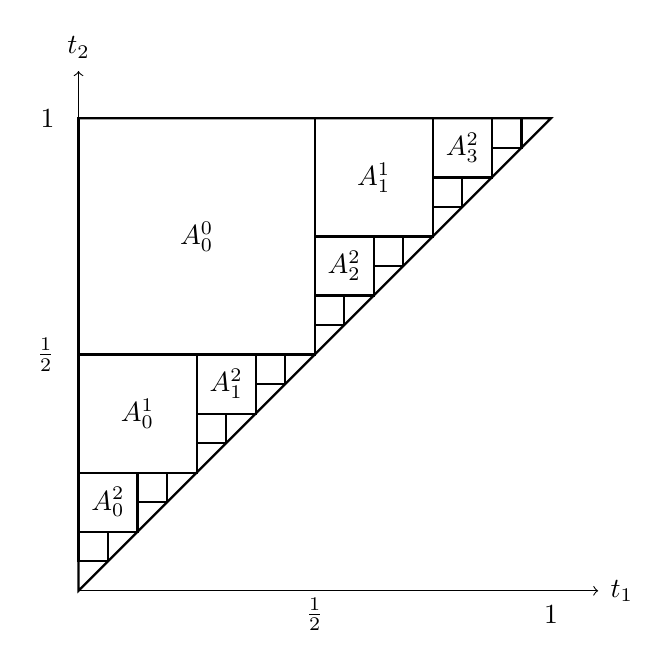
\begin{tikzpicture}[scale=6]
  % Triangle boundary
  \draw[thick] (0,0) -- (1,1) -- (0,1) -- cycle;

  % Level 0 squares
  \draw[thick] (0,1/2) rectangle (1/2,1); % A_0^0
  \node at (0.25,0.75) {$A_0^0$};

  \draw[thick] (0,1/4) rectangle (1/4,1/2); % A_0^1
  \node at (1/8,1/4+1/8) {$A_0^1$};

  \draw[thick] (1/2,3/4) rectangle (3/4,1); % A_1^1
  \node at (1-1/4-1/8,1-1/8) {$A_1^1$};

  % Recursive pattern inside 1
  \foreach \i in {0,1,2,3} {
    \pgfmathsetmacro\x{(\i) / 4}
    \pgfmathsetmacro\y{\x + 1/8}
    \pgfmathsetmacro\xend{\x + 1/8}
    \pgfmathsetmacro\yend{(\i + 1) / 4}
    \pgfmathsetmacro\xmid{(\x + \xend)/2}
    \pgfmathsetmacro\ymid{(\y + \yend)/2}
    \draw[thick] (\x,\y) rectangle (\xend,\yend); 
    \node at (\xmid, \ymid) {$A^2_\i$};
  }

  % Recursive pattern inside 2
  \foreach \i in {0,1,2,3,4,5,6,7} {
    \pgfmathsetmacro\x{(\i) / 8}
    \pgfmathsetmacro\y{\x + 1/16}
    \pgfmathsetmacro\xend{\x + 1/16}
    \pgfmathsetmacro\yend{(\i + 1) / 8}
    \draw[thick] (\x,\y) rectangle (\xend,\yend);
  }
    


  % Axes
  \draw[->] (0,0) -- (1.1,0) node[right] {};
  \draw[->] (0,0) -- (0,1.1) node[above] {};

  % Axis labels
  \node at (1.15,0) {$t_1$};
  \node at (0.5,-0.05) {$\frac{1}{2}$};
  \node at (1,-0.05) {$1$};
  \node at (0, 1.15) {$t_2$};
  \node at (-0.03,0.5) [anchor=east] {$\frac{1}{2}$};
  \node at (-0.03,1) [anchor=east] {$1$};

\end{tikzpicture}
\caption{Four steps of the partition of $\mathcal{T}_2\cap[0,1]^2$ by squares $A^k_l$ ($k=0,1,2,3$).}
\label{fig:A_l^k partition}
\end{figure}

Before defining the renormalised self-intersection local time, we introduce a proposition (proof adapted from \cite{RandomWalkIntersections:}) that connects the two intersection local times we constructed. This is precisely the idea that we described above: we divide the Brownian motion and consider intersections between independent Brownian motions. For the remainder of the section, let $\beta$ be the $2$-multiple self-intersection local time of a standard planar Brownian motion $B$, and let $\alpha$ be the intersection local time of two independent standard planar Brownian motions.

\begin{proposition}\label{prop:beta2_deq_alpha2_for_intervals}
    For any $0\leq a < b < c$:
    \[
    \beta([a,b]\times[b,c])\deq\alpha([0,b-a]\times[0,c-b]).
    \]
\end{proposition}
\begin{proof}
    For $\epsilon>0$ and $b<b'<c$ using the definitions in \cref{eq:beta_ep_local_time_formula_for_sets} and \cref{eq:alpha_ep_local_time_formula_for_sets} we have:
    \begin{align*}
        \beta&_\epsilon([a,b]\times[b',c]) = \int_{\R^2}dy\int_a^b\delta_y^\epsilon(B(s))ds\int_{b'}^c\delta_y^\epsilon(B(r))dr\\
        &= \int_{\R^2}dy\int_{b'-b}^{b'-a}\delta_y^\epsilon(B_1(u)+B(b'))du\int_0^{c-b'}\delta_y^\epsilon(B_2(v)+B(b'))dv \\
        &= \int_{\R^2}dx\int_{b'-b}^{b'-a}\delta_x^\epsilon(B_1(u))du\int_0^{c-b'}\delta_{x}^\epsilon(B_2(v))dv = \alpha_{\epsilon}([b-b',b'-a]\times[0,c-b'])
    \end{align*}
    where we used the changes of variables $u=b'-s$, $v=r-b'$ and $x=y-B(b')$, and defined $B_1(t)=B(b'-t)-B(b')$ and $B_2(t)=B(t+b')-B(b)$, which are two independent standard planar Brownian motions.

    Finally, taking $\epsilon\downarrow0$ and $b'\downarrow b$ we have the desired result.
\end{proof}
\begin{remark}\label{rmk:equality_beta_alpha_intervals}
    In particular, $\beta(A_l^l)\deq \alpha([0,2^{-(k+1)}]^2)\deq 2^{-(k+1)}\alpha([0,1]^2)$, where in the last equality in distribution we used \cref{prop:properties_alpha_local_time} iii).
\end{remark}

Finally, we can define the renormalisation. The next theorem can be found in \cite{LeGallSomeProperties} Chapter VIII, but the proof has been significantly expanded to provide additional clarity to its arguments.

\begin{theorem}[Renormalised self-intersection local time]\label{thm:renormalised-local-time}
    For any Borel subset $A$ of $\mathcal{T}$, consider the mapping $A\mapsto \gamma(A)$ defined by:
    \[
        \gamma(A) = \sum_{k=0}^\infty 
            \left( 
                \sum_{l=0}^{2^k-1} \left( \beta(A\cap A_l^k) - \expect\left[\beta(A\cap A_l^k)\right] \right)
            \right).
    \]
    
    The series on the RHS converges a.s. and in $\mathcal{L}^2$. We call this mapping the \textnormal{renormalised self-intersection local time}.
\end{theorem}
\begin{proof}
      For any fixed $k$, $\beta(A\cap A_l^k)$ for $l=0,\dots,2^k-1$ are independent since each of them only depends on the increments of $B$ between disjoint intervals of time. If we define 
      \[
      X_k = \sum_{l=0}^{2^k-1} \left( \beta(A\cap A_l^k) - \expect\left[\beta(A\cap A_l^k)\right] \right),
      \]
      notice that $\expect[X_k]=0$ for any $k\geq 0$. These two observations imply that $\expect[X_kK_j]=0$ for any $k,j\geq0$.

      Then, by \cref{rmk:equality_beta_alpha_intervals}, 
      \begin{align*}
      \text{Var}&\left(\sum_{l=0}^{2^k-1}\beta(A\cap A^k_l) \right) = \sum_{l=0}^{2^k-1}\text{Var}\left( \beta(A\cap A^k_l)\right)\leq \sum_{l=0}^{2^k-1}\expect\left[ \beta(A^k_l)^2 \right] \\
      &= 2^k\expect\left[2^{-k-1}\alpha([0,1]^2)^2\right] = 2^{-k-2}\expect[\alpha([0,1]^2)^2] = C 2^{-k},
      \end{align*}
      writing $C=\expect[\alpha(([0,1]^2)^2]/4$, which is a constant.

      Now we are ready to prove the statements. Let $S_n = \sum_{k=0}^nX_k$.
    
      \begin{itemize}
          \item \textbf{$\mathcal{L}^2$ convergence}
            We want to show that $\expect[(S_n-S_m)^2]\to0$ as $m,n\to\infty$. By the observations above, $$\expect[S_n^2]=\sum_{k=0}^n\expect[X_k^2].$$
            We finish by observing that 
            $$\expect[(S_n-S_m)^2] = \sum_{k=m+1}^n\expect[X_k^2]\to0$$
            as $m,n\to\infty$ since 
            \[
            \sum_{k=0}^\infty\expect[X_k^2] = \sum_{k=0}^\infty\text{Var}(X_k) =  \sum_{k=0}^\infty\text{Var}\left(\sum_{l=0}^{2^k-1}\beta(A\cap A^k_l) \right) 
            \leq C < \infty.
            \]
          
          \item \textbf{a.s. convergence}
            Similarly, we show $|S_n-S_m|\to0$ a.s. as $m,n\to\infty$. For any $\epsilon>0$ and naturals $m>n$, by Kolmogorov's maximal inequality,
            \[
            \prob(\max_{m<k\leq n}|S_k-S_m|>\epsilon) \leq \frac{\operatorname{Var}(S_n-S_m)}{\epsilon^2}.
            \]

            Now, letting $n\to\infty$, we have:
            \[
            \prob(\sup_{k>m}|S_k-S_m|>\epsilon)\leq\frac{\sum_{k=m+1}^\infty\operatorname{Var(X_k)}}{\epsilon^2} \to 0
            \]
            as $m\to\infty$, since, as above, $\sum_{k=0}^\infty\operatorname{Var(X_k)}<\infty$.

            Lastly, we finish the proof by observing that
            \[
            \prob\left(\sup_{k,n>m}|S_k-S_n|>2\epsilon\right)\leq 
            \prob\left( \sup_{k>m}|S_k-S_m|>\epsilon \right) \to 0
            \]
            as $m\to\infty$.
          
      \end{itemize}
\end{proof}

\subsubsection{Behaviour between hitting times of multiple points}

We want to study in generality how the path between hitting times of a multiple point behaves, and whether a $p$-multiple point is likely to also have multiplicity $p+1$, as discussed in the previous section. To accomplish this goal, we require one more technical theorem regarding intersection local times. For any integer $p\geq2$ we write $\beta_p$ for the random measure constructed in \cref{thm:beta_local_time_construction}. 

For $0\leq u\leq v$ set $B_u^v(t) = B((u+t)\wedge v)-B(u)$,
\begin{comment}
\begin{align*}
&B_u^v(t) = B((u+t)\wedge v)-B(u)=
\begin{cases}
    B(u + t) - B(u) & \text{if } 0 \leq t \leq v - u \\
    B(v) - B(u)     & \text{if }  v - u < t,
\end{cases}\\
%&B_v^u(t) = B_v^u(t)=B((v-t)\vee u)-B(v) =
%\begin{cases}
%    B(v - t) - B(v) & \text{if } 0 \leq t \leq v - u \\
%    B(u) - B(v)     & \text{if }  v - u < t,
%\end{cases}
\end{align*}
\end{comment}
which are random continuous functions $\R_\geq\to\R^2$. $B_u^v(t)$ represents a Brownian trajectory starting at 0 `paused' after reaching $B(v)-B(u)$ at time $v-u$, and $B_v^u(t)$ a backward Brownian trajectory `paused' at $B(v)-B(u)$. Here `paused' refers to the fact that for all $t\geq v-u$, we assign the same value to the process.

We also set $L_r(t)$ for a Brownian loop with initial point $0$ and length $r$, and `paused' at 0, in the same sense as above, meaning we use the convention $L_r(t)=0$ for all $t\geq r$.

Lastly, for any process $X$, set $X^T(t)=X(t\wedge T)$ for the stopped process at $T$.

\begin{theorem}\label{thm:beta-local-time-and-loops}
    For $p\geq2$, any $A\in\mathcal{B}(\mathcal{T}_p)$, and any non-negative measurable function $F:\mathcal{C}(\R_\geq\to\R^2)^{p+1}\to\R$, we have:
    \begin{align}\label{eq:expectation-beta-local-time-and-loops}
        \begin{split}
            &\expect\left[
                        \int_A\beta_p(dt_1\dots dt_p)F(B_0^{t_1}, B_{t_1}^{t_2}, \dots, B_{t_p}^{\infty})
                    \right]\\
            &=\int_A \frac{dt_1\dots dt_p}{(2\pi)^{p-1}(t_2-t_1)\dots(t_p-t_{p-1})} 
            \expect \left[
                        F(W^{t_1}, L^{(1)}_{t_2-t_1}, \dots, L^{(p-1)}_{t_p-t_{p-1}}, \tilde{W})
                    \right]
        \end{split}
    \end{align}
    where $W$ and $\tilde W$ are independent standard planar Brownian motions, independent of $L^{(j)}_{t_{j+1}-t_j}$ for all $j=1,\dots, p-1$, and $L^{(j)}_{t_{j+1}-t_j}$ are all Brownian loops as above.

    Furthermore, let $H$ be a Borel subset of $\mathcal{C}(\R_\geq\to\R^2)^{p+1}$ such that
    \[
        \prob   \left(
                    (W^{t_1}, L^{(1)}_{t_2-t_1}, \dots, L^{(p-1)}_{t_p-t_{p-1}}, \tilde{W})\in H
                \right)
        = 1,
    \]
    for almost all $(t_1,\dots,t_p)\in\mathcal{T}_p$ with respect to the Lebesgue measure $dt_1\dots dt_p$. Then, almost surely, for almost all $(t_1,\dots,t_p)\in\mathcal{T}_p$ with respect to the measure $\beta_p(dt_1\dots dt_p)$,
    \[
        (B_0^{t_1}, B_{t_1}^{t_2}, \dots, B_{t_p}^{\infty})\in H
    \]
\end{theorem}
\begin{proof}
    Using monotone class arguments we can assume $F$ is continuous and bounded, and $A$ is a compact rectangle of $\mathcal{T}_p$. Then from \cref{thm:beta_local_time_construction}, and writing $\beta_{\epsilon,p}$ for the $\epsilon$ approximation for $p$ points, we have:
    \begin{align*}
    \expect&
        \left[
            \int_AF(B_0^{t_1},B_{t_1}^{t_2},\dots,\beta_{t_p}^\infty)\beta_p(dt_1\dots dt_p)
        \right]
        =
        \lim_{\epsilon\downarrow0}\expect
            \left[ 
            \int_AF(B_0^{t_1},B_{t_1}^{t_2},\dots,\beta_{t_p}^\infty)\beta_{\epsilon,p}(dt_1\dots dt_p) 
            \right]\\
    &= \lim_{\epsilon\downarrow0}\int_A 
    \expect\left[ \int_{\R^2}\ind_{D_\epsilon(y)}(B(t_1))\dots\ind_{D_\epsilon(y)}(B(t_p))F(B_0^{t_1},\dots,B_{t_p}^{\infty})dy \right]\frac{dt_1\dots dt_p}{(\pi\epsilon^2)^p}\\
    &= \lim_{\epsilon\downarrow0}\int_A  m(D_\epsilon(B({t_1}))\cap \dots\cap D_\epsilon(B({t_p}))) \expect\left[ F(B_0^{t_1},\dots,B_{t_p}^{\infty}) \right] \frac{dt_1\dots dt_p}{(\pi\epsilon^2)^p},
    \end{align*}
    where $m$ is the Lebesgue measure.

    Observe that $m(D_\epsilon(B(t_1))\cap \dots\cap D_\epsilon(B({t_p})))
    =m(D_\epsilon(0)\cap D_\epsilon(B({t_2})-B({t_1}))\cap \dots\cap D_\epsilon(B({t_p})-B(t_1))),
    %=m(D_\epsilon(0)\cap D_\epsilon(y_2)\cap \dots\cap D_\epsilon(y_p))
    $
     since the Lebesgue measure is translation invariant. Also, setting $B({t_j})-B({t_1})=y_j$ for $j=2,\dots,p$, observe $y_j=B({t_j})-B({t_{j-1}})+B({t_{j-1}})-\dots+B({t_2})-B({t_1})$. Then it is easy to see that $B({t_j})-B({t_{j-1}})=y_{j}-y_{j-1}$.

    It follows that
    \begin{align*}
    \expect&
        \left[
            \int_AF(B_0^{t_1},B_{t_1}^{t_2},\dots,B_{t_p}^\infty)\beta_{\epsilon,p}(dt_1\dots dt_p)
        \right]\\
        &=\int_A dt_1\dots dt_p\int_{\|y_j-y_{j-1}\|<2\epsilon}dy_2\dots dy_p \frac{m(D_\epsilon(0)\cap \dots\cap D_\epsilon(y_p))}{(\epsilon^2\pi)^{p}}\prod_{j=2}^{p}p_{t_j-t_{j-1}}(y_{j-1},y_j) \\ 
        &\expect\left[ F(B_0^{t_1},\dots,B_{t_{p-1}}^{t_p})\middle|B(t_p)-B(t_{p-1})=y_p-y_{p-1},\dots, B(t_2)-B(t_1)=y_2 \right].
    \end{align*}

    Notice $\epsilon\downarrow0$ implies $y_j\to0$ for $j=2,\dots,p$ and then
    \[
    \lim_{y_j\to0,\forall j} \expect\left[ F(B_0^{t_1},\dots,B_{t_p}^\infty)\middle|B(t_k)-B(t_{k-1})=y_{k}-y_{k-1}, \forall k \right] = \expect\left[ F(W^{t_1},L^{(1)}_{t_2-t_1},\dots,L^{(p-1)}_{t_p-t_{p-1}},\tilde{W}) \right].
    \] Also, 
    \[
    \lim_{\epsilon\downarrow0}\prod_{j=2}^pp_{t_j-t_{j-1}}(y_{j-1},y_j)=\frac{1}{(2\pi)^{p-1}(t_2-t_1)\dots(t_p-t_{p-1})}.
    \]

    Moreover, one can show that $\int_{\R^2} m(D_\epsilon(0)\cap \dots\cap D_\epsilon(y_p))dy_2\dots dy_p = (\pi\epsilon^2)^{p}$.

    Putting everything together, 
    \begin{align*}
        \expect&
        \left[
            \int_AF(B_0^{t_1},B_{t_1}^{t_2},\dots,\beta_{t_p}^\infty)\beta_p(dt_1\dots dt_p)
        \right]\\
        &=\int_A \frac{dt_1\dots dt_p}{(2\pi)^{p-1}(t_2-t_1)\dots(t_p-t_{p-1})} 
            \expect \left[
                        F(W^{t_1}, L^{(1)}_{t_2-t_1}, \dots, L^{(p-1)}_{t_p-t_{p-1}}, \tilde{W})
                    \right],
    \end{align*}
    as we wanted to prove.

    Finally, we need to show the second assertion of the theorem. Take $F$ to be the indicator function $\ind_{H^c}$. Then, by the work above:
    \begin{align*}
        \expect&
        \left[
            \int_A\ind_{H^c}(B_0^{t_1},B_{t_1}^{t_2},\dots,\beta_{t_p}^\infty)\beta_p(dt_1\dots dt_p)
        \right] = \int_A \prob\left( (B_0^{t_1},B_{t_1}^{t_2},\dots,\beta_{t_p}^\infty)\in H^c \right)\beta_p(dt_1\dots dt_p) \\
        &=\int_A \frac{1}{(2\pi)^{p-1}(t_2-t_1)\dots(t_p-t_{p-1})} 
            \expect \left[
                        \ind_{H^c}(W^{t_1}, L^{(1)}_{t_2-t_1}, \dots, L^{(p-1)}_{t_p-t_{p-1}}, \tilde{W})
                    \right]dt_1\dots dt_p\\
        &= \int_A \frac{1}{(2\pi)^{p-1}(t_2-t_1)\dots(t_p-t_{p-1})} 
            \prob\left((W^{t_1}, L^{(1)}_{t_2-t_1}, \dots, L^{(p-1)}_{t_p-t_{p-1}}, \tilde{W})\in H^c\right)dt_1\dots dt_p,
    \end{align*}
    which completes the proof.
\end{proof}

\begin{remark}
     \cref{thm:beta-local-time-and-loops} is useful because it describes how the process behaves between hitting times of a multiple point. In particular, it provides insight into why our previous construction of a double point did not behave as expected: that is not a typical multiple point in the sense of the intersection local time.
\end{remark}
\begin{remark}
    The theorem above is also providing a weak version of the Markov property at the hitting times of a multiple point. Indeed, the second assertion states that any property that holds almost surely for independent Brownian motions and loops will also hold before or after the successive hitting times of a typical multiple point. This becomes very relevant in the next section.
\end{remark}

Going back to our third question, now we can show that $p+1$ multiple points are non common among $p$-multiple points.

\begin{proposition}\label{prop:impossible_p+1_multiple_points}
    Almost surely, for almost all $(t_1,\dots,t_p)$ with respect to $\beta_p$, the point $B({t_1})=\dots=B({t_p})=x\in\R^2$ is not a $(p+1)$-multiple point.
\end{proposition}
\begin{remark}\label{remark:theorem_impossible_p+1_multiple_points}
    The idea behind this proof is that we will consider a set of functions $H$ that allows for $p$-multiple points, but not for $p+1$-multiple points. We will then apply the previous theorem to find that all points of multiplicity $p$ belong to $H$ almost surely, and thus they are not $p+1$-multiple points.
\end{remark}
\begin{proof}
    For $\varphi\in\mathcal{C}(\R_\geq\to\R^2)$, let $\zeta(\varphi)\defeq\inf\{t>0:\varphi \text{ is constant on } [t,\infty)\}$,
    with the convention that $\inf\emptyset=\infty$.

    Then define the set
    \[
        H = \left\{
        \begin{aligned}
        (\varphi_0,\varphi_1,\dots,\varphi_p)\in\mathcal{C}(\R_{\geq}\to\R^2)^{p+1} :\quad
        &\forall t\in[0,\zeta(\varphi_0))\quad \varphi_0(t)\neq\varphi_0(\zeta(\varphi_0))\quad  \\
        \text{and for } j=1,\dots,p,\quad &\forall t\in(0,\zeta(\varphi_j))\quad \varphi_j(t)\neq\varphi_j(0)
        \end{aligned}
        \right\}
    \]

    Recall that planar Brownian motion does not hit points, i.e. for $B$ a Brownian motion and any $y\in\R^2$, $\prob(\exists t>0:B(t)=y)=0$. Then, it follows that, using the same notation as in \cref{thm:beta-local-time-and-loops}, with probability 1, $X^{t_1}$ does not hit $X(t_1)$ before $t_1$, the loops $L^{(j)}_{t_j-t_{j+1}}$ and $\tilde X$ do not go back to their starting points. Therefore, $H$ satisfies the assumptions of the theorem.

    As discussed in \cref{remark:theorem_impossible_p+1_multiple_points}, this implies that $x$ is a.s. not a $(p+1)$-multiple point, since the definition of $H$ does not allow it.
\end{proof}

Notice that \cref{thm:existence-p-multiple-points} and \cref{prop:impossible_p+1_multiple_points} give the existence of points of multiplicity exactly $p$, almost surely. In the next section we will see a much stronger result that also proves this fact.

\subsection{Points of infinite multiplicity}
In this section we prove the main result for which we have been working towards: planar Brownian motion has points that are visited infinitely often. Not only that, it has points of uncountable multiplicity. 

The strategy we will follow for the proof relies on finding a double point and then looking near it for points of doubling multiplicity in such a way that the limit of these points is a point of infinite multiplicity. To do this, we want to apply the results from \cref{sect:local-times}, for which we need an additional lemma that states, accounting for the consequences of \cref{thm:beta-local-time-and-loops}, that for typical multiple points, if we consider paths at times shortly after and shorty before its hitting times, these paths behave like independent Brownian motions. With this, we will be able to use the properties of the $\alpha$ measure we constructed in \cref{sect:alpha_local_time}.

\begin{lemma}\label{lemma:positive_beta_2p_from_p_point}
    Almost surely, for $p\geq 2$, almost all $(t_1,\dots,t_p)\in\mathcal{T}_p$ with respect to $\beta_p$, and any $\delta>0$ small enough so that the intervals do not overlap,
    \[
    \beta_{2p}((t_1-\delta,t_1)\times(t_t,t_1+\delta)\times\dots\times(t_p-\delta, t_p)\times(t_p,t_p+\delta))>0.
    \]
\end{lemma}
\begin{proof}
    Consider an arbitrary compact rectangle $R\subset\mathcal{T}_p$. Then we can find a sequence $\epsilon_k\downarrow0$ such that 
    \begin{equation}\label{eq:lemma_positive_beta_2p_from_p_point_beta_limit}
    \beta_p(R)=\lim_{k\to\infty}\beta_{\epsilon_k,p}(R)\quad\text{a.s.}
    \end{equation} 

    Since all self-intersection local times converge as $\epsilon\downarrow0$, we can further assume that the same sequence works for any $p$ and any rectangle with rational coordinates. A monotone class type argument shows that the previous limit holds for any rectangle of $\mathcal{T}_p$, for any $p$.

    Similarly, let $\alpha_p$ be the intersection local time of $p$ independent standard planar Brownian motions, as defined in \cref{sect:alpha_local_time}. We can also assume that the same sequence satisfies 
   \begin{equation}\label{eq:lemma_positive_beta_2p_from_p_point_lim_alpha}
       \alpha_p(R')=\lim_{k\to\infty}\alpha_{\epsilon_k,p}(R'),\quad\text{a.s.}
   \end{equation} 
   for all compact rectangles $R'\subset(\R_\geq)^p$ 

   We now define the continuous functions $f_0,f_1,\dots,f_p\in\mathcal{C}(\R_\geq\to\R^2)$ and set, as before, $\zeta_j\defeq\zeta(f_j)=\inf\{t>0:\text{ }f_j\text{ is constant in }[t,\infty)\}$. Then we set:
   \begin{align*}
    l_\delta(f_0,f_1,\dots,f_p)=
    \liminf_{k\to\infty}\int_{[0,\delta]^p}\varphi_{\epsilon_k,2p}(&f_0(\zeta_0-t_1), f_1(t_2), f_1(\zeta_2-t_2),\dots,\\
    &f_{p-1}(t_{2(p-1)}),f_{p-1}(\zeta_{p-1}-t_{2p-1}),f_p(t_{2p}))dt_1\dots dt_p,
   \end{align*}
   if $\zeta_j<\infty$ for all $j\in\{0,1,\dots,p-1\}$, and otherwise we set $l_\delta(f_0,f_1,\dots,f_p)=0$.
   In the definition above we used
   \[
    \varphi_{\epsilon,2p}(z_1,\dots,z_p)=\int_{\R^2}\prod_{j=1}^{2p}\delta_y^\epsilon(z_j)dy.
   \]
   as in \cref{sect:local-times}.

   The set
   \[
   H=\{(f_0,f_1,\dots,f_p):l_\delta(f_0,f_1,\dots,f_p)>0\quad\forall\delta>0\}
   \]
   satisfies the assumptions of \cref{thm:beta-local-time-and-loops}. Indeed, observe that by the absolute continuity stated in \cref{lemma:equivalence-law-loops-bm}, $l_\delta$ being positive for Brownian motions is enough, which follows from \cref{eq:lemma_positive_beta_2p_from_p_point_lim_alpha} and \cref{prop:properties_alpha_local_time} iv).

   Therefore, with probability 1 for almost all $(s_1,\dots,s_p)\in\mathcal{T}_p$ with respect to $\beta_p$:
   $$(B_0^{s_1},B_{s_1}^{s_2},\dots,B_{s_{p-1}}^{s_p},B_{s_p}^\infty)\in H.$$ 

   Finally, the desired result follows using \cref{eq:lemma_positive_beta_2p_from_p_point_beta_limit} and the definition of $\beta_{\epsilon,2p}$.

\end{proof}

\subsubsection{The Cantor set and order type}
Now we have all the main tools to prove the existence of points of infinite multiplicity. However, in order to make all the steps rigorous, let us take one last excursion to define and introduce some results from other areas of mathematics that are used in the proof.

\begin{definition}[Cantor set]
    The Cantor set, denoted here as $\Cantor$, is a subset of $\R$ that is normally constructed by iteratively removing the middle third of the set. More formally, let $\Cantor_0=[0,1]$, then setting \[\Cantor_n=\frac{\Cantor_{n-1}}{3}\cup\left(\frac{2}{3}+\frac{\Cantor_{n-1}}{3}\right),\]
    the Cantor set is defined by
    \[
    \Cantor = \lim_{n\to\infty}\Cantor_n=\bigcap_{n=0}^\infty\Cantor_n.
    \]
    Moreover, we say a set is a Cantor set if it is homeomorphic to $\Cantor$.
\end{definition}

Now, let us introduce, without proof, some useful results regarding the Cantor set. The following statements and their proofs can be found in \cite{CantorSet}.

%\begin{proposition}
%    Every perfect complete metric space contains a subspace that is homeomorphic to the Cantor set.
%\end{proposition}

\begin{proposition}\label{prop:Cantor_set_uncountable}
    The Cantor set is uncountable and of Lebesgue measure zero.
\end{proposition}

\begin{theorem}[Brouwer]\label{thm:brouwer}
    Every totally disconnected compact perfect metric space is homeomorphic to the Cantor set. Equivalently, every totally disconnected compact metric space without isolated points is a Cantor set.
\end{theorem}

To finalise this section, we introduce the concept of order type, that appears in the statement of the main theorem.
\begin{definition}[Order type]
    We say two compact subsets $K,K'\subset\R$ have the same \textnormal{order type} if there exists an increasing homeomorphism $\varphi:\R\to\R$ such that $\varphi(K)=K'$.
\end{definition}
\begin{remark}
    Since $\varphi$ is invertible by definition, order type is symmetric, i.e. if there exists a decreasing homeomorphism $\phi$ such that $\phi(K)=K'$, take $\varphi(x)=\phi^{-1}(x)$ and exchange the roles of $K$ and $K'$.
\end{remark}

We provide some examples of sets that have the same order type, and some that do not:
\begin{example}
Sets with the same order type.
    \begin{enumerate}[a)]
        \item Any set $A$ and an affine transformation of it $B=f(A)$. For example, $[0,1]$ and $[1,10]$, the cantor set $\Cantor$ and $\Cantor + 1$, or the integers $\Z$ and even numbers $\Z$.
        \item Finite ordered sets of the same cardinality. Indeed, let \( A = \{a_1, \dots, a_p\} \) and \( B = \{b_1, \dots, b_p\} \), where the elements are listed in increasing order. Then the map \( \varphi(a_i) = b_i \) is an order-preserving bijection. Since any such bijection between finite subsets of \( \mathbb{R} \) can be extended to an increasing homeomorphism \( \varphi: \mathbb{R} \to \mathbb{R} \) (e.g., by linear interpolation between the points and affine extensions outside).
    \end{enumerate}
Sets with different order type.
    \begin{enumerate}[a)]
        \item The Cantor set $\Cantor$ and $[0,1]$. Even if both are uncountable sets of $\R$, as we will see $\Cantor$ is totally disconnected, whereas $[0,1]$ is connected. Since $\varphi$ preserves topological properties, there can not exist such transformation between the two sets.
        \item The Cantor set $\Cantor$ and $\Cantor\cup\{p\}$ for an isolated point $p\in\R$. Once again because they have different topological properties.
    \end{enumerate}
\end{example}

\subsubsection{Main result}
We return to multiple points in Brownian motion. Let $B$ be a Brownian motion in $\R^2$ started at $0$.
\begin{theorem}
    Let $K$ be a totally disconnected compact subset of $\R$. Then with probability 1 there exists a point $z\in\R^2$ such that $\{t\geq0:B(t)=z\}$ has the same order type as $K$.
\end{theorem}

\begin{remark}
    This theorem is remarkably general as it provides the existence of points of exactly any finite multiplicity, points of countable multiplicity, and points of uncountable multiplicity. But not only that, we can also find points of uncountable multiplicity were the set of times has the same order type as a Cantor set and a series of isolated points, which we saw is different from the Cantor set alone.
\end{remark}

Since we have already proved the existence of points of any finite multiplicity, we will restrict our proof to the infinite case. In particular, we will first prove that we can find a set of times that contains a Cantor set, which implies the existence of points of uncountable multiplicity, and then we will prove that we can construct this set of times in a way that it is exactly a Cantor set. For clarity, we will treat these versions as separate theorems, but in reality, the first is a simplification of the second. We reproduce both proofs here because understanding the arguments in \cref{thm:main_result_v1} makes it easier to follow the more general proof of \cref{thm:main_result_v2}

This first result is proved in \cite{LeGallSomeProperties}.
\begin{theorem}\label{thm:main_result_v1}
    With probability 1, there exists a point $z\in\R^2$ of uncountable multiplicity, in particular, $\{t\geq0:B(t)=z\}$ contains a Cantor set.
\end{theorem}
\begin{proof}
    As previously stated, we will iteratively construct a sequence of points $(z_n)_n$ that converge to the desired $z$.

    \begin{itemize}
        \item \textbf{First step}.

        Set $t^0_1=1/2$, $z_0=B(t_1^0)$, $\delta_0=1/4$.

    For any $\delta>0$ we have:
    \[
        \beta_2((t_1^0-\delta,t_1^0) \times (t_1^0,t_1^0+\delta)) \deq \alpha_2((0,\delta)^2)>0,
    \]
    where we used \cref{prop:beta2_deq_alpha2_for_intervals} and \cref{prop:properties_alpha_local_time}. Therefore, taking \(\delta=\delta_0\) above, there exists $(t_1^1,t_2^1)\in(t_1^0-\delta_0,t_1^0)\times(t_1^0,t_1^0+\delta_0)=(\frac{1}{4},\frac{1}{2})\times(\frac{1}{2},\frac{3}{4})\subset\mathcal{T}_2$ such that $B(t_1^1)=B(t_2^1)=z_1$.

    Then by \cref{lemma:positive_beta_2p_from_p_point}, for any $\delta>0$ small enough, 
    \[
        \beta_4((t_1^1-\delta,t_1^1)\times(t_1^1,t_1^1+\delta)\times(t_2^1-\delta,t_2^1)\times(t_2^1,t_2^1+\delta))>0.
    \]

    \item \textbf{Induction step.}

    At the $n$-th step we have found 
    \[
    (t^n_1,\dots, t^n_{2^n})\in (t^{n-1}_1-\delta_{n-1},t^{n-1}_1) \times (t^{n-1}_1, t^{n-1}_1+\delta_{n-1}) \times \dots \times (t^{n-1}_{2^{n-1}}-\delta_{n-1},t^{n-1}_{2^{n-1}}) \times (t^{n-1}_{2^{n-1}}, t^{n-1}_{2^{n-1}}+\delta_{n-1})
    \]
    such that $z_n=B(t^n_1)=\dots=B(t_{2^n}^n)$. 
    
    By applying \cref{lemma:positive_beta_2p_from_p_point} again, we have, for any $\delta>0$:
    \[
        \beta_{2^{n+1}}((t_1^{n}-\delta,t_1^n)\times (t_{1}^n, t_{1}^n+\delta) \times\dots\times (t_{2^n}^{n}-\delta,t_{2^n}^n) \times (t_{2^n}^n, t_{2^n}^n+\delta))>0.
    \]
    Once again, this is valid, in particular, for $\delta_n\defeq\frac{1}{4}\left(\delta_{n-1}\wedge \min(t^n_i-t^n_{i-1}:i=2,\dots,2^n)\right)$.

    Proceeding like before, we find 
    \[
    (t_1^{n+1},\dots,t_{2^{n+1}}^{n+1})\in(t^{n}_1-\delta_{n},t^{n}_1) \times (t^{n}_1, t^{n}_1+\delta_{n}) \times \dots \times (t^{n}_{2^{n}}-\delta_{n},t^{n}_{2^{n}}) \times (t^{n}_{2^{n}}, t^{n}_{2^{n}}+\delta_{n})
    \]
    satisfying $z_{n+1}\defeq B(t_1^{n+1}) = \dots = B(t^{n+1}_{2^{n+1}})$, and we can set $$\delta_{n+1}\defeq\frac{1}{4}\left(\delta_{n}\wedge \min(t^{n+1}_i-t^{n+1}_{i-1}:i=2,\dots,2^{n+1})\right).$$  Now we are ready to apply \cref{lemma:positive_beta_2p_from_p_point} again and build the next iteration.
    \end{itemize}

    Note that $\min\left(|t_i^{n+1}-t_{i-1}^{n+1}|:i=2,\dots,2^{n+1}\right)\leq 2\delta_n\leq \frac{1}{2^n}$. That is, we can find a Cauchy sequence $\tau_j=t^j_{k_j}$ for some $k_j\in\{1,\dots,2^j\}$, and therefore $\tau_j$ converges to some $\tau$. By continuity of Brownian motion, the sequence $(z_n)_n$ converges to some $z=B(\tau)\in\R^2$.

    Consider now the closed set 
    \[
    S=\bigcap_{n=1}^\infty \overline{\left( \bigcup_{m=n}^\infty \left\{t_j^m:j\in \{ 1,\dots,2^m \} \right\} \right)},
    \]
    where $\overline{X}$ denotes the closure of the set $X$. Note that for any $t\in S$, $B(s)=z$, as, for example, it contains the limit points of sequences like the one constructed above. Therefore, the set $\{ t\geq 0: B(t)=z\}$ contains $S$.

    Finally, $S$ is compact, as it is closed and bounded in $\R$. Moreover, it is totally disconnected, and it has no isolated points (it is dense), as can be seen by its definition. By Brouwer's \cref{thm:brouwer}, $S$ is a Cantor set. By \cref{prop:Cantor_set_uncountable} we have that the point $z$ has uncountable multiplicity and we finish the proof.
    
\end{proof}

Before continuing, it is worth taking some time to examine the main ideas of the previous proof. Note that it involves no technical estimate, as we have included all technicalities within the local times that we constructed in previous sections. 

The basic idea we followed is: we start with a double point $z_1$. We then use that the 4 paths around the double point (i.e. $B(t_1^1-\delta,t_1^1)$, \(B(t_1^1,t_1^1+\delta)\), \(B(t_2^1-\delta,t_2^1)\), and \(B(t_2^1,t_2^1+\delta)\)) behave like independent Brownian motions (\cref{lemma:positive_beta_2p_from_p_point} and \cref{prop:beta2_deq_alpha2_for_intervals}) and therefore have an intersection (\cref{prop:properties_alpha_local_time}), which is a $4$-multiple point. We continued iteratively and constructed points of doubling multiplicity that converge to a point $z$. 

Finally, we argued that this point $z$ is visited at a set of times that contains a Cantor set. To do so rigorously, we used topological arguments, but notice that, intuitively, at each iteration we are discarding the endpoints of the intervals from being in the next iteration. This will remind the reader of removing the middle third in the canonical construction of the Cantor set.

The following version can be found in \cite{LeGallFrench}, theorem 5.1. Here, it has been translated to English.
\begin{theorem}\label{thm:main_result_v2}
    With probability 1, there exists a point $z\in\R^2$ such that $\{t\geq0:B(t)=z\}$ is a Cantor set.
\end{theorem}
\begin{proof}
    The idea is the same as in \cref{thm:main_result_v1}, but now we require our sequences $t^n$, $z_n$, $\delta_n$, and the new $\eta_n$ to be more general. We divide the proof into three steps. First we introduce some notation and show that we can reduce our work to proving a special case. Then we show how we can construct the sequences mentioned above. Lastly, we show that what we found in step 2 does indeed satisfy all the requirements to finish the proof.

    \begin{itemize}
    \item \textbf{Step 1.}

        For any integer $n\geq0$, we set $\Omega_n=\{0,1\}^n$ with the convention that $\Omega_0=\{\emptyset\}$. Let $\mathcal{A}$ be the set of subsets $A\subset\Omega=\bigcup_{n=0}^\infty\Omega_n$ verifying:
        \begin{enumerate}[i)]
            \item $\emptyset\in A$
            \item If $(x_1,\dots,x_n)\in A$ then $(x_1,\dots,x_n,0)\in A$.
            \item If $(x_1,\dots,x_n)\in A$ for $n\geq1$, then $(x_1,\dots,x_{n-1})\in A$.
        \end{enumerate}

        In other words, any $A\in\mathcal{A}$ is a set of finite binary sequences that contains the empty set, is stable under $0$ expansion, and contains all prefixes of its sequences.

        To provide a more intuitive understanding, one can see $\Omega_n$ as the $n$-th level of a binary tree with root $\emptyset$ and, as we go down, each node appends a $0$ (for left branch, for example) or a $1$. Then $A$ is a set of nodes that contains all the left-children, and all the parents of its elements. This is exemplified in \cref{fig:binary-tree-example}.

        \begin{figure}[ht]
        \centering
        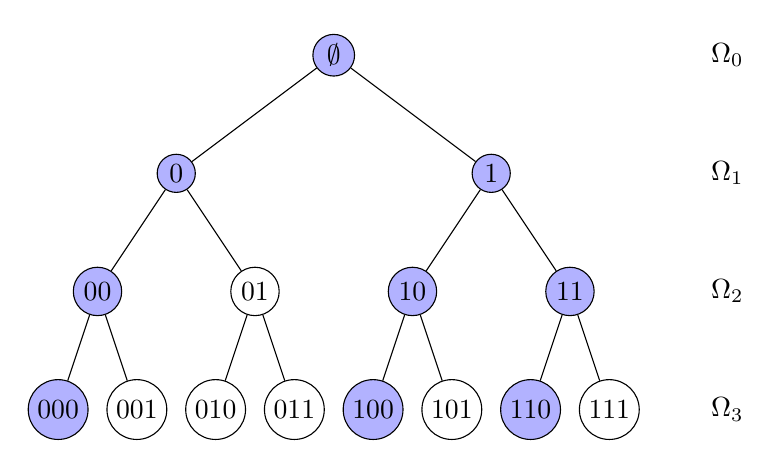
\begin{tikzpicture}[
            level distance=1.5cm,
            level 1/.style={sibling distance=4cm},
            level 2/.style={sibling distance=2cm},
            level 3/.style={sibling distance=1cm},
            every node/.style={circle,draw,inner sep=2pt},
            selected/.style={fill=blue!30}
          ]
        
          % Tree structure
          \node[selected] (root) {$\emptyset$}
            child { node[selected] {0}
              child { node[selected] {00} 
                child { node[selected] {000} }
                child { node {001} }
              }
              child { node {01} 
                child { node {010} }
                child { node {011} }
              }
            }
            child { node[selected] {1}
              child { node[selected] {10} 
                child { node[selected] {100} }
                child { node {101} }
              }
              child { node[selected] {11} 
                child { node[selected] {110} }
                child { node {111} }
              }
            };
        
          % Level labels
          \node[draw=none] at ($(root)+(5,0)$) {$\Omega_0$};
          \node[draw=none] at ($(root)+(5,-1.5)$) {$\Omega_1$};
          \node[draw=none] at ($(root)+(5,-3)$) {$\Omega_2$};
          \node[draw=none] at ($(root)+(5,-4.5)$) {$\Omega_3$};
        
        \end{tikzpicture}
        \caption{A binary tree with a subset \( A \subset \mathcal{A} \) highlighted in blue. Each level of the tree corresponds to a $\Omega_n$.}
        \label{fig:binary-tree-example}
        \end{figure}
        
        Let $I=\{0,1\}^\N$, with the convention that $0\notin\N$. For $u=(u_1,\dots,u_n,\dots)\in I$ and all $n\geq 0$ we write the truncation $[u]_n=(u_1,\dots,u_n)\in\Omega_n$. Similarly, for $m>n$ and $x\in\Omega_m$, we write $[x]_n=(x_1,\dots,x_n)\in\Omega_n$.

        For any $A\in\mathcal{A}$, we define $I_A=\{u\in I: \forall n\geq 0, [u]_n\in A\}$ the set of infinite binary sequences whose finite prefixes all live in $A$. Note that it is a non-empty compact subset of $I$.

        One can show that if $K$ is a totally disconnected non-empty compact subset of $(0,\infty)$, like the Cantor set, then we can find a set $A\in\mathcal{A}$ such that $K$ and $I_A$ have the same order type. Thanks to this observation, we are reduced to showing that for any set $A\in\mathcal{A}$ there almost surely exists a point $z\in\R^2$ and an increasing homeomorphism $\varphi:I_A\to B^{-1}(z)$, with $B^{-1}(z)=\{t\in\R_\geq:B(t)=z\}$.

    \item \textbf{Step 2.}

        Fix $A\in\mathcal{A}$ and for all $n\geq 0$ set $A_n=A\cap\Omega_n$ the set of sequences of length $n$. Going back to the tree visualisation, $A_n$ is the level $n$ of the subtree that corresponds to $A$. For example, in \cref{fig:binary-tree-example}, $A_2=\{00,10,11\}$. We also set $m_n=\text{Card}(A_n)$ for the cardinality of $A_n$.

        Our goal is to construct a collection of times $(t_x,x\in A)\subset(0,\infty)$ such that for all $n\geq0$, $z_n=B(t_x)$ for all $x\in A_n$. To make explicit the iteration we are working with, we will write $t^n_x$ for $x\in A_n$. Notice that this is what we did in \cref{thm:main_result_v1} where we were using $A_n=\Omega_n$ and at each iteration we found times $t^n_x$ for $x\in\Omega_n$, understanding each $x$ as the value it represents in binary base.

        For all $\epsilon>0$ and all families $(b_x,x\in A_n)$ of positive numbers, we write $\Delta_\epsilon(b_x,x\in A_n)$ the set of collections $(c_x,x\in A_{n+1})$ such that:
        \begin{enumerate}
            \item If $x=(x',0)$ then $b_{x'}-\epsilon<c_x<b_{x'}$,
            \item If $x=(x',1)$ then $b_{x'}<c_x<b_{x'}+\epsilon$,
        \end{enumerate} 
        which is precisely what we did in \cref{thm:main_result_v1} with the intervals.

        Now we inductively construct: 
        \begin{itemize}
            \item a family $(t_x,x\in A)\subset(0,1)$,
            \item two sequences $(\delta_n)_{n\geq0}$ and $(\eta)_{n\geq0}$ of strictly positive numbers converging to $0$,
            \item a sequence $(z_n)_{n\geq0}\subset\R^2$,
        \end{itemize}
        so that the following properties hold:
        \begin{enumerate}[a)]
            \item $(t^n_x,x\in A_n)=B^{-1}(z_n)\cap[0,1]$,
            \item $(t^n_x,x\in A_n)\in\Delta_\epsilon(t^{n-1}_x,x\in A_{n-1})$,
            \item $\delta_n<\frac{1}{8}\inf \left(|t^{n-1}_x-t^{n-1}_y|:x,y\in A_{n-1}\right)$,
            \item $\delta_n<\frac{1}{2}\delta{n-1}$,
            \item if $s\in[0,1]$ such that $|s-t^n_x|>2^{-n}$ for all $x\in A_{n}$, then $|B(s)-z_n|>2\eta_n$,
            \item for all $s,t\in[0,1]$ with $|s-t|<2\delta_n$, we have $|B(t)-B(s)|<\eta_{n-1}$,
            \item for all $\epsilon>0$, $\beta_{m_{n+1}}\left(\Delta_\epsilon(t_x^n,x\in A^n)\right)>0$.
        \end{enumerate}

        As in \cref{thm:main_result_v1}, we do the construction inductively:
        \begin{itemize}
            \item \textbf{Base case}.

            Set $t_\emptyset=1/2$, $z_0=B(t_\emptyset)$, and $\epsilon_0=\eta_0=1$.

            We begin by choosing $\epsilon_1$ in such a way that properties (c), (d), and (f) hold. Separately treating the two possible cases $A_1=\{0\}$ and $A_1=\{0,1\}$, we construct a family $(t^1_x,x\in A_1)$ in such a way that (a), (b) and (b) are satisfied for $n=1$. Once again, the argument for (g) will come from a similar result to \cref{lemma:positive_beta_2p_from_p_point} (see \cite{LeGallFrench} Lemma 4.1). Finally, taking into account (a) we choose $\eta_n>0$ small enough so that (e) is verified.

            \item \textbf{Inductive case}.

            Now let $p\geq 2$ and suppose that we have built for all $n\leq p-1$ a family $(t^n_x,x\in A_n)$ and have extended the sequences with $z_n$, $\delta_n$ and $\eta_n$, satisfying properties (a)-(g).

            As above, we choose $\delta_p$ taking into account (c), (d), and (f) at order $p$. 

            Next, using property (g) written to order $p-1$, we can find a family $(t_x^p,x\in A_p)\in\Delta_{\epsilon_p}(t_x^{p-1},x\in A_{p-1})$ in such a way that (a) and (g) are satisfied at order $p$, for which we use the same arguments as before. 

            Finally, thanks to (a) we can choose $\eta_p>0$ in such a way that (e) is satisfied. This completes our construction.
            
        \end{itemize}

        Note that properties (b) and (c) show that for all $n$, the application $x\mapsto t_x^n$ for $x\in A_n$ is increasing (taking the ordering from left to right in the tree representation, i.e. the natural order in binary base). In fact, this was used implicitly in our construction.

        Furthermore, using (b) and (d) we see that if $m\leq n$ and $x\in A_m$, $y\in A_n$ are such that $[y]_m=x$, we have $|t^m_x-t^n_y|\leq2\delta_{n+1}$, from which, according to (f), we get $|B(t^m_x)-B(t^n_y)|\leq\eta_n$.

        Now we set 
        \[
        S=\bigcap_{n=0}^\infty \overline{\left( \bigcup_{m=n}^\infty \{ t^m_x,x\in A_m \} \right)}.
        \]

        The previous remarks show that we can define an application $\varphi:I_A\to S$ by setting $\varphi(u)=\lim_{n\to\infty}t^n_{[u]_n}$ for all $u\in I_A$. Then property (a) implies that $B$ takes the same value in all points of $S$: $z=\lim_{n\to\infty}z_n$.
 
    
    \item \textbf{Step 3.}

    Now it remains to show that $S=B^{-1}(z)$ and that $\varphi$ is an increasing homeomorphism, which, together with Step 1, will mean that $S$ has the same order type as $K$, which we can take to be a Cantor set.

    We start by establishing $S=B^{-1}(z)$. The Markov property of Brownian motion implies that it is enough to show $S=B^{-1}(z)\cap[0,1]$. Let $t\in[0,1]\setminus S$, we will see $t\notin B^{-1}(z)$. We can choose $n$ big enough that for all $x\in A_n$, $|t-t^n_x|>2^{-n}$. Then property (e) implies that $|B(t)-z_n|>2\eta_n$. On the other hand, properties (b), (d), and (f) result in $|z_n-z|\leq\eta_n$, from where we conclude, by the triangle inequality, 
    \[
    |B(t)-z|\geq|B(t)-z_n|-|z_n-z|>\eta_n,
    \]
    and thus $B(t)\neq z$.

    Now we show that $\varphi$ is an increasing homeomorphism. The fact it is increasing follows from the observation above that the application $x\mapsto t^n_x$ for $x\in A_n$ is increasing. Then, properties (b), (d), and (f) lead to the fact that $\varphi$ is continuous and injective. To show that $\varphi$ is surjective, let $t\in S$. By definition, we can find a sequence $(x(n))_n$ with $x(n)\in A_{k_n}$ and $k_n\to\infty$ such that 
    \[
    t=\lim_{n\to\infty}t_{x(n)}^{k_n}.
    \]
    Notice that then we have 
    \[
        t_{x(n)}^{k_n}-t^{k_m}_{x(m)}\underset{m,n\to\infty}{\to}0,
    \]
    which means that for any integer $p$ there exists a unique element $x_p\in A_p$ such that for all $n$ big enough, $[x(n)]_p=x_p$. If $u\in I_A$ is defined by $[u]_p=x_p$ for all p, then we have $\varphi(u)=a$, which completes the proof.
    
    \end{itemize}
\end{proof}

\section{Conclusion and other directions}
In this essay, we explored the structure of planar Brownian motion through the lens of intersection local times, culminating in a proof of the existence of points of infinite multiplicity. Beginning with the construction of local times for multiple intersections, we saw how these objects capture intricate features of the Brownian path, and how they serve as rigorous tools for quantifying self-intersection. We also analysed how their name reflects their connection to the Brownian local times and occupation measures. These express the intuitive idea of measuring how often the path returns to the same location, making them natural instruments in the study of path self-intersections. In both cases we proceeded by constructing local times via global approximations. Instead, they can be derived as natural measures supported on the relevant sets, as we hinted in the end of \cref{sect:from_brownian_local_time_to_intersection}. This alternative route, while leading to the same objects, provides a conceptually distinct perspective and constitutes a natural extension or parallel approach to the ideas developed here. It is of independent mathematical interest and worthy of further exploration.

While our focus was on multiple points in Brownian motion, intersection local times are of broader interest, extending to other problems and disciplines. In particular, they appear in models from polymer physics and quantum field theory. Polymer models, for example, describe the geometric shape of the polymer using suitable random paths, like Brownian motion. This makes it desirable to define a random variable that measures the number of multiple self-intersections up to a fixed time. In this setting, the renormalised self-intersection local time that we saw in \cref{sect:double_points} is indispensable. Le Gall explores this renormalisation more generally in Chapters X and XI of \cite{LeGallSomeProperties}. Beyond its applications in physics, renormalisation can also be applied to asymptotic expansions of the area of the Wiener sausage. All these ideas and applications also constitute a natural expansion of this essay.

The existence of points of infinite multiplicity reveals the extraordinary recurrence and fractal-like complexity of Brownian motion. This is further exemplified by Le Gall's proof, which relates these times to the Cantor set. Certainly, the process in which we iteratively found denser sets of times in which the Brownian motion is at the same point, shows the self-similar and complex nature of Brownian motion. The key point to take away from it should be how we successfully related intuitive ideas about multiple points, and the paths leading to and from them, to the rigour of intersection local times.

In \cref{sect:multiple_points}, we saw two proofs of the existence of finitely-multiple points. Similarly, our approach to uncountably infinite multiple points is not unique. In \cite{BrownianMotion}, Chapter 9, Mörters and Peres follow a comparable strategy, by constructing a binary tree of time intervals. The paths from the root downwards represent sequences of nested intervals, whose intersection will be mapped to a single point by the Brownian motion. However, they avoid the use of intersection local times by introducing other technical estimates.

The methods developed in this essay illustrate the richness of probability theory and suggest many directions for further exploration, such as analogous questions for other classes of stochastic processes. Admittedly, Rosen and Yor introduced Tanaka-like formulas for intersection local times and explored self-intersections, including in more general diffusions and Lévy processes (\cite{LeGallSomeProperties}, Chapter VIII, Bibliographical notes).


%This is how you can start a new page
\vfill \eject

%%%%%%%%%%%%%%%%%%%%%%%%%%%%%%%%%%%%%%%%%%%%%%%%%%%%%%%%%%%%%%%%%%%%%%
%                                                                             
% REFERENCES
%                                                                             
%%%%%%%%%%%%%%%%%%%%%%%%%%%%%%%%%%%%%%%%%%%%%%%%%%%%%%%%%%%%%%%%%%%%%%

% List any references you have used below. You can list papers in your preferred style, e.g. as below.
% To cite a paper in your text, use \cite{}.

% If you prefer, you can list your papers in a separate .bib file. This is often much more efficient and easier to change later.
% An explanation of how to do this can be found at https://www.overleaf.com/learn/latex/Bibliography_management_with_bibtex.
% When submitting the essay, you must upload your .bib file alongside this .tex file.

\bibliographystyle{amsplain}
\bibliography{refs}


%\begin{thebibliography}{99}
%\bibitem{examplebib}
%Author (Year) \emph{Title}, Publisher
%\bibitem{Burkill} Burkill, J.C. (1962) \emph{A First Course in Mathematical Analysis}, CUP
%\bibitem{Ledermann} Ledermann, W. and Weir, A.J. (1996) \emph{An Introduction to Group Theory %(2nd edition)}, Longman 
%\bibitem{Warner} Warner, F.W. (1970) \emph{Foundations of Differentiable Manifolds and Lie %Groups}, Springer Graduate Texts in Mathematics 
%\bibitem{Schutz} Schutz, B. (2022) \emph{A First Course in General Relativity (3rd edition)}, CUP  
%\bibitem{Lovelock} Lovelock, D. (1971) \emph{The Einstein Tensor and Its Generalizations}, Journal of Mathematical Physics 
%{\bf 12} (3): 498–501
%\bibitem{Stillwell}
%Stillwell, J. (2016) \emph{Elements of Mathematics}, Princeton University Press

%\end{thebibliography}

\end{document}

